\documentclass[12pt]{article}

% --- Encoding and fonts (Times-like text with matching math) ---
\usepackage[utf8]{inputenc}
\usepackage[T1]{fontenc}
\usepackage{amsmath}
\usepackage{amssymb}
\usepackage{newtxtext}
\usepackage{newtxmath}
\usepackage{microtype}

% --- Graphics, colour, tables ---
\usepackage{graphicx}
\usepackage{xcolor}
\usepackage{float}
\usepackage{multirow}
\usepackage{rotating}

% --- Units and numbers ---
\usepackage{siunitx}
\sisetup{group-separator={,}, group-minimum-digits=4}

% --- Page layout and spacing ---
\usepackage[letterpaper, margin=1in]{geometry}
\usepackage{setspace}
\doublespacing
\usepackage{caption}
\captionsetup{labelsep=period, labelfont=bf, font={footnotesize,singlespacing}}
\renewcommand{\figurename}{Fig}
\interfootnotelinepenalty=10000

% --- Bibliography (numbered, IOP style via iopart-num.bst) ---
\usepackage{cite}

% --- Cross-references by name (for unnumbered section headings) ---
\usepackage{nameref}

% --- Hyperlinks and linked ORCID icons (loaded after other packages) ---
\usepackage{hyperref}
\usepackage{orcidlink}
\definecolor{linknavy}{rgb}{0,0,0.5}
\hypersetup{
  colorlinks=true,
  linkcolor=linknavy,
  citecolor=linknavy,
  urlcolor=linknavy,
  pdftitle={Local goodness-of-fit measures for neural decoding},
  pdfauthor={Sirui Zeng, Alison E. Comrie, Loren M. Frank, Uri T. Eden, Eric L. Denovellis},
}


% Generated by scripts/emit_reported_values.py --- do not edit by hand.
%
% Every value below is read from the canonical figure summaries:
%   figures/main/figure03_summary.json (schema 7)
%   figures/main/figure04_summary.json (schema 4)
%   figures/supplementary/figure04_supplement_summary.json (schema 1)
%   figures/supplementary/figure03_sensitivity_summary.json (schema 1)
% source_tree_sha256: f6cc646bebe61f90e940353b53fe709de7c932c0d87d5e4acc00df9ac9ed53a7
%
% Regenerate with: uv run python scripts/emit_reported_values.py

% --- Simulation study (Figure 3) --- computed from the simulated data
\newcommand{\SimNRealizations}{100}                         % realizations.count
\newcommand{\SimFirstSeed}{1}                               % realizations.first_seed
\newcommand{\SimLastSeed}{100}                              % realizations.last_seed
\newcommand{\SimNCalibration}{100}                          % calibration.count
\newcommand{\SimCalibrationSeedFirst}{1001}                 % calibration.first_seed
\newcommand{\SimCalibrationSeedLast}{1100}                  % calibration.last_seed
\newcommand{\SimCalibrationSteps}{6000}                     % calibration.steps_per_session
\newcommand{\SimCalibrationEvents}{289278}                  % calibration.n_pooled_events
\newcommand{\SimHpdThreshold}{0}                            % flag_rules.hpd_overlap.threshold
\newcommand{\SimKlThreshold}{4.2}                           % flag_rules.kl_divergence.threshold
\newcommand{\SimCalibrationTail}{0.34\%, 2.6\%, and 4.8\%}  % calibration.rank_pvalue_tail_percentages at alphas 0.01, 0.05, 0.10
\newcommand{\SimMatchedNullTail}{0.35\%, 2.6\%, and 4.7\%}  % matched_null_rank_pvalue_tail_percentages at alphas 0.01, 0.05, 0.10
\newcommand{\SimKlClipEvents}{2126394}                      % kl_clip_impact.evaluation.n_events
\newcommand{\SimKlClipDiffering}{54}                        % kl_clip_impact.evaluation.n_differing_events
\newcommand{\SimKlClipMaxDifference}{1.0}                   % kl_clip_impact.evaluation.max_difference (nats)
\newcommand{\SimKlClipFlagChanges}{0}                       % kl_clip_impact.evaluation.n_flag_changes
\newcommand{\SimKlClipNullDiffering}{0}                     % kl_clip_impact.calibration.n_differing_events
\newcommand{\SimNullHpdFlag}{1.6}                           % calibration.pooled_null_flag_percentages.hpd_overlap
\newcommand{\SimNullPvalueFlag}{2.6}                        % calibration.pooled_null_flag_percentages.predictive_pvalue
\newcommand{\SimNullKlFlag}{1.0}                            % calibration.pooled_null_flag_percentages.kl_divergence
\newcommand{\SimMatchedNullFlagMin}{1}                      % min over metrics of median_flag_percentages[:, matched_null]
\newcommand{\SimMatchedNullFlagMax}{3}                      % max over metrics of median_flag_percentages[:, matched_null]
\newcommand{\SimRecoveryFlagMin}{1}                         % min over metrics of median_flag_percentages[:, recovery]
\newcommand{\SimRecoveryFlagMax}{3}                         % max over metrics of median_flag_percentages[:, recovery]
\newcommand{\SimRemapFlagMin}{19}                           % min over metrics of median_flag_percentages[:, remap]
\newcommand{\SimRemapFlagMax}{24}                           % max over metrics of median_flag_percentages[:, remap]
\newcommand{\SimHistoryFlagMin}{1}                          % min over metrics of median_flag_percentages[:, history_dependent]
\newcommand{\SimHistoryFlagMax}{2}                          % max over metrics of median_flag_percentages[:, history_dependent]
\newcommand{\SimReplayFlagMin}{1}                           % min over metrics of median_flag_percentages[:, replay]
\newcommand{\SimReplayFlagMax}{3}                           % max over metrics of median_flag_percentages[:, replay]
\newcommand{\SimDriftFlagMin}{8}                            % min over metrics of median_flag_percentages[:, drift]
\newcommand{\SimDriftFlagMax}{14}                           % max over metrics of median_flag_percentages[:, drift]
\newcommand{\SimReflectFlagMin}{1}                          % min over metrics of median_flag_percentages[:, reflected_map]
\newcommand{\SimReflectFlagMax}{3}                          % max over metrics of median_flag_percentages[:, reflected_map]
\newcommand{\SimRemapHpdFlag}{23}                           % median_flag_percentages[hpd_overlap, remap]
\newcommand{\SimMatchedNullHpdFlag}{1.5}                    % median_flag_percentages[hpd_overlap, matched_null]
\newcommand{\SimMatchedNullPvalueFlag}{2.6}                 % median_flag_percentages[predictive_pvalue, matched_null]
\newcommand{\SimMatchedNullKlFlag}{0.95}                    % median_flag_percentages[kl_divergence, matched_null]
\newcommand{\SimSparseHpdFlag}{0}                           % median_flag_percentages[hpd_overlap, sparse_population]
\newcommand{\SimSparsePvalueFlag}{0}                        % median_flag_percentages[predictive_pvalue, sparse_population]
\newcommand{\SimSparseKlFlag}{56}                           % median_flag_percentages[kl_divergence, sparse_population]
\newcommand{\SimSparsePooledHpdFlag}{0.99}                  % pooled_flag_percentages[hpd_overlap, sparse_population]
\newcommand{\SimSparsePooledPvalueFlag}{1.4}                % pooled_flag_percentages[predictive_pvalue, sparse_population]
\newcommand{\SimRemapPooledMin}{28}                         % min over metrics of pooled_flag_percentages[:, remap]
\newcommand{\SimRemapPooledMax}{33}                         % max over metrics of pooled_flag_percentages[:, remap]
\newcommand{\SimRemapHpdQLow}{12}                           % 25th percentile over realizations of flag_percentages_by_realization[hpd_overlap, remap]
\newcommand{\SimRemapHpdQHigh}{52}                          % 75th percentile over realizations of flag_percentages_by_realization[hpd_overlap, remap]
\newcommand{\SimMatchedNullError}{1.8}                      % median_decoding_accuracy[median_absolute_error, matched_null]
\newcommand{\SimMatchedNullCoverage}{96}                    % median_decoding_accuracy[filtered_hpd_coverage_percent, matched_null]
\newcommand{\SimRecoveryError}{1.8}                         % median_decoding_accuracy[median_absolute_error, recovery]
\newcommand{\SimRecoveryCoverage}{95}                       % median_decoding_accuracy[filtered_hpd_coverage_percent, recovery]
\newcommand{\SimRemapError}{42}                             % median_decoding_accuracy[median_absolute_error, remap]
\newcommand{\SimRemapCoverage}{1}                           % median_decoding_accuracy[filtered_hpd_coverage_percent, remap]
\newcommand{\SimHistoryError}{1.9}                          % median_decoding_accuracy[median_absolute_error, history_dependent]
\newcommand{\SimHistoryCoverage}{94}                        % median_decoding_accuracy[filtered_hpd_coverage_percent, history_dependent]
\newcommand{\SimReplayError}{37}                            % median_decoding_accuracy[median_absolute_error, replay]
\newcommand{\SimReplayCoverage}{5}                          % median_decoding_accuracy[filtered_hpd_coverage_percent, replay]
\newcommand{\SimDriftError}{8.0}                            % median_decoding_accuracy[median_absolute_error, drift]
\newcommand{\SimDriftCoverage}{36}                          % median_decoding_accuracy[filtered_hpd_coverage_percent, drift]
\newcommand{\SimReflectError}{47}                           % median_decoding_accuracy[median_absolute_error, reflected_map]
\newcommand{\SimReflectCoverage}{2}                         % median_decoding_accuracy[filtered_hpd_coverage_percent, reflected_map]
\newcommand{\SimSparseError}{4.2}                           % median_decoding_accuracy[median_absolute_error, sparse_population]
\newcommand{\SimSparseCoverage}{98}                         % median_decoding_accuracy[filtered_hpd_coverage_percent, sparse_population]
\newcommand{\SimRemapFilteredSize}{11}                      % median_decoding_accuracy[median_filtered_hpd_size, remap]
\newcommand{\SimMatchedNullPredictiveSize}{11}              % median_decoding_accuracy[median_predictive_hpd_size, matched_null]
\newcommand{\SimSparsePredictiveSize}{26}                   % median_decoding_accuracy[median_predictive_hpd_size, sparse_population]
\newcommand{\SimReplayRepresentedError}{1.3}                % replay_represented_accuracy.median[median_absolute_error]
\newcommand{\SimReplayRepresentedCoverage}{97}              % replay_represented_accuracy.median[filtered_hpd_coverage_percent]
\newcommand{\SimMatchedNullRateHz}{484}                     % phase_ordinary_spike_rates_hz.median[matched_null]
\newcommand{\SimHistoryRateHz}{488}                         % phase_ordinary_spike_rates_hz.median[history_dependent]
\newcommand{\SimSparseEventsMedian}{12}                     % sparse_population.median_sparse_cell_event_count
\newcommand{\SimSparseEventsMin}{4}                         % min of sparse_population.sparse_cell_event_counts_by_realization
\newcommand{\SimSparseEventsMax}{25}                        % max of sparse_population.sparse_cell_event_counts_by_realization
\newcommand{\SimHpdPercentile}{1st}                         % threshold_provenance.hpd_overlap.quantile
\newcommand{\SimKlPercentile}{99th}                         % threshold_provenance.kl_divergence.quantile
\newcommand{\SimPredictiveCutoff}{0.05}                     % threshold_provenance.predictive_pvalue.cutoff

% --- Simulation study (Figure 3) --- recorded configuration
\newcommand{\SimTrackLength}{100}                  % position_max
\newcommand{\SimPositionMin}{0}                    % position_min
\newcommand{\SimNPlaceCellsWord}{eleven}           % len(place_field_centers)
\newcommand{\SimNNeuronsWord}{twenty-two}          % len(place_field_centers) + len(sparse_place_field_centers)
\newcommand{\SimPlaceFieldSpacing}{10}             % place_field_centers spacing
\newcommand{\SimPlaceFieldStd}{10}                 % place_field_std
\newcommand{\SimRateScale}{5}                      % place_field_rate_scale
\newcommand{\SimPeakCountPerStep}{0.20}            % place_field_rate_scale / (place_field_std * sqrt(2 pi))
\newcommand{\SimPeakRateHz}{200}                   % peak expected count per step at 1 ms/step, in Hz
\newcommand{\SimPredictionStepStd}{0.5}            % prediction_step_std
\newcommand{\SimNSparseCellsWord}{eleven}          % len(sparse_place_field_centers)
\newcommand{\SimNSparseCellsWordCap}{Eleven}       % len(sparse_place_field_centers), sentence-initial
\newcommand{\SimSparseFieldStd}{2}                 % sparse_place_field_std
\newcommand{\SimSparseActiveRateHz}{5}             % sparse_cell_peak_rate_per_step, in Hz
\newcommand{\SimSparseMultiplierMin}{0.5}          % min(sparse_cell_rate_multipliers)
\newcommand{\SimSparseMultiplierMax}{2}            % max(sparse_cell_rate_multipliers)
\newcommand{\SimSparseBaselineFractionPercent}{1}  % 100 * sparse_cell_baseline_rate_fraction
\newcommand{\SimDurationSteps}{42000}              % phase_boundaries[-1]
\newcommand{\SimDurationSeconds}{42}               % phase_boundaries[-1] at 1 ms/step
\newcommand{\SimNPhasesWord}{ten}                  % len(phase_boundaries)
\newcommand{\SimRemapStart}{6000}                  % phase_boundaries[0]
\newcommand{\SimRemapEnd}{10000}                   % phase_boundaries[1]
\newcommand{\SimRecoveryOneEnd}{14000}             % phase_boundaries[2]
\newcommand{\SimHistoryEnd}{18000}                 % phase_boundaries[3]
\newcommand{\SimRecoveryTwoEnd}{22000}             % phase_boundaries[4]
\newcommand{\SimDriftEnd}{26000}                   % phase_boundaries[5]
\newcommand{\SimRecoveryThreeEnd}{30000}           % phase_boundaries[6]
\newcommand{\SimReflectEnd}{34000}                 % phase_boundaries[7]
\newcommand{\SimRecoveryFourEnd}{38000}            % phase_boundaries[8]
\newcommand{\SimSparseEnd}{42000}                  % phase_boundaries[9]
\newcommand{\SimReplayStart}{19000}                % replay_start_fraction within clean recovery 2
\newcommand{\SimReplayEnd}{21000}                  % replay_end_fraction within clean recovery 2
\newcommand{\SimReplayRateScale}{20}               % replay_place_field_rate_scale
\newcommand{\SimReplayGainWord}{four}              % replay_place_field_rate_scale / place_field_rate_scale
\newcommand{\SimReplaySpeedCap}{0.5}               % replay_speed_per_step
\newcommand{\SimReplayMaxSpeed}{0.10}              % track length / transitions per sweep leg
\newcommand{\SimRemapDisplacementWord}{three}      % min displacement in place_field_remapping
\newcommand{\SimDriftMomentum}{0.88}               % drift_momentum
\newcommand{\SimDriftVelocityStd}{1.1}             % prediction_step_std / sqrt(1 - drift_momentum^2)
\newcommand{\SimRefractoryMs}{1}                   % history_refractory_steps at 1 ms/step
\newcommand{\SimBurstStartMs}{2}                   % history_burst_window[0] at 1 ms/step
\newcommand{\SimBurstEndMs}{10}                    % history_burst_window[1] at 1 ms/step
\newcommand{\SimBurstFactorWord}{three}            % history_burst_factor
\newcommand{\SimHistoryGain}{0.512}                % history_rate_matching_gain

% --- Simulation study (Figure 3) --- sensitivity settings
\newcommand{\SimSensitivityCoverageRows}{95\% coverage (main setting) & 0.00 & 1.6 & 2.6 & 1.0 & 23 & 11 & 56 \\ 50\% coverage & 0.00 & 38 & 2.6 & 1.0 & 68 & 56 & 56 \\ 80\% coverage & 0.00 & 11 & 2.6 & 1.0 & 43 & 28 & 56 \\ Reflected continuous walk (95\%) & 0.00 & 1.4 & 2.4 & 1.0 & 41 & 11 & 60 \\}  % figure03_sensitivity_summary settings
\newcommand{\SimSensitivitySparseRows}{Ordinary ensemble at 0.005 of its rate & 22 & 12 & 4 & 0 & 0 & 32 \\ Ordinary ensemble at 0.01 of its rate & 31 & 12 & 2 & 0 & 0 & 21 \\ Ordinary ensemble at 0.05 of its rate & 110 & 12 & 3 & 11 & 1 & 5 \\ Sparse cells at half rate & 6 & 6 & 0 & 0 & 0 & 75 \\}    % figure03_sensitivity_summary sparse settings
\newcommand{\SimSparseOrdinaryScales}{0.005, 0.01, and 0.05}                                                                                                                                                                                                                                                   % sparse_control_ordinary_rate_scale sensitivity values
\newcommand{\SensCoverageFiftyNullHpd}{38}                                                                                                                                                                                                                                                                     % settings[hpd_coverage_0.5].calibration.pooled_null_flag_percentages.hpd_overlap
\newcommand{\SensContinuousRemapHpd}{41}                                                                                                                                                                                                                                                                       % settings[continuous_reflected_trajectory].median_flag_percentages[hpd_overlap, remap]
\newcommand{\SensContinuousSparseKl}{60}                                                                                                                                                                                                                                                                       % settings[continuous_reflected_trajectory].median_flag_percentages[kl_divergence, sparse_population]
\newcommand{\SensCoverageEightyNullHpd}{11}                                                                                                                                                                                                                                                                    % settings[hpd_coverage_0.8].calibration.pooled_null_flag_percentages.hpd_overlap

% --- Hippocampal recording (Figure 4) --- computed from the recording
\newcommand{\RecNUnits}{203}                       % dataset.n_units
\newcommand{\RecHpdFlaggedContinuous}{18790}       % flag_confusions[hpd_overlap]: a_only + both
\newcommand{\RecHpdRescued}{17289}                 % flag_confusions[hpd_overlap].a_only
\newcommand{\RecHpdRescuedPercent}{92}             % flag_confusions[hpd_overlap].rescue_rate
\newcommand{\RecHpdNewlyFlagged}{176}              % flag_confusions[hpd_overlap].b_only
\newcommand{\RecPvalueFlaggedContinuous}{33954}    % flag_confusions[predictive_pvalue]: a_only + both
\newcommand{\RecPvalueRescued}{9373}               % flag_confusions[predictive_pvalue].a_only
\newcommand{\RecPvalueRescuedPercent}{28}          % flag_confusions[predictive_pvalue].rescue_rate
\newcommand{\RecPvalueNewlyFlagged}{1706}          % flag_confusions[predictive_pvalue].b_only
\newcommand{\RecNEvents}{870018}                   % flag_confusions[hpd_overlap].n
\newcommand{\RecHpdFlaggedContinuousPercent}{2.2}  % flag_confusions[hpd_overlap]: (a_only + both) / n

% --- Hippocampal recording (Figure 4 supplement) --- computed from the recording
\newcommand{\RecDurationMinutes}{24}                                                                                                                                                                                                                                                   % rate_and_behavior.duration_seconds / 60
\newcommand{\RecNActiveUnits}{182}                                                                                                                                                                                                                                                     % rate_and_behavior.n_active_units
\newcommand{\RecNZeroEventUnits}{21}                                                                                                                                                                                                                                                   % rate_and_behavior.n_zero_event_units
\newcommand{\RecNPositionBins}{248}                                                                                                                                                                                                                                                    % region_size_and_broadening.by_coverage[0.95].n_position_bins
\newcommand{\RecHpdCutoffPercent}{5}                                                                                                                                                                                                                                                   % 100 * region_size_and_broadening.hpd_flag_threshold
\newcommand{\RecContRegionAll}{13}                                                                                                                                                                                                                                                     % median 95% Continuous predictive region size, all events
\newcommand{\RecContRegionRescued}{8}                                                                                                                                                                                                                                                  % median 95% Continuous predictive region size, rescued events
\newcommand{\RecFragRegionAll}{144}                                                                                                                                                                                                                                                    % median 95% Continuous-Fragmented predictive region size, all events
\newcommand{\RecFragRegionRescued}{110}                                                                                                                                                                                                                                                % median 95% Continuous-Fragmented predictive region size, rescued events
\newcommand{\RecLikelihoodRegion}{228}                                                                                                                                                                                                                                                 % median 95% likelihood region size, all events
\newcommand{\RecLikelihoodOutsidePercent}{8}                                                                                                                                                                                                                                           % 100 * (1 - median likelihood region / n_position_bins)
\newcommand{\RecMixWeightA}{0.02}                                                                                                                                                                                                                                                      % uniform_mixture[0.02].uniform_weight
\newcommand{\RecMixRemovedA}{25}                                                                                                                                                                                                                                                       % uniform_mixture[0.02].fraction_original_flags_removed
\newcommand{\RecMixWeightB}{0.05}                                                                                                                                                                                                                                                      % uniform_mixture[0.05].uniform_weight
\newcommand{\RecMixRemovedB}{79}                                                                                                                                                                                                                                                       % uniform_mixture[0.05].fraction_original_flags_removed
\newcommand{\RecMixWeightC}{0.06}                                                                                                                                                                                                                                                      % uniform_mixture[0.06].uniform_weight
\newcommand{\RecMixRemovedC}{95}                                                                                                                                                                                                                                                       % uniform_mixture[0.06].fraction_original_flags_removed
\newcommand{\RecMixWeightD}{0.10}                                                                                                                                                                                                                                                      % uniform_mixture[0.1].uniform_weight
\newcommand{\RecMixRemovedD}{100}                                                                                                                                                                                                                                                      % uniform_mixture[0.1].fraction_original_flags_removed
\newcommand{\RecMixNewMax}{24}                                                                                                                                                                                                                                                         % max over mixture weights < 1 of n_new_flags
\newcommand{\RecCovEightyContFlagged}{221434}                                                                                                                                                                                                                                          % by_coverage[0.8].continuous.n_flagged
\newcommand{\RecCovEightyRescuedPercent}{41}                                                                                                                                                                                                                                           % by_coverage[0.8].rescue_fraction
\newcommand{\RecCovFiftyContFlagged}{566882}                                                                                                                                                                                                                                           % by_coverage[0.5].continuous.n_flagged
\newcommand{\RecCovFiftyContFlaggedPercent}{65}                                                                                                                                                                                                                                        % by_coverage[0.5].continuous.n_flagged / n_events
\newcommand{\RecCovFiftyRescuedPercent}{15}                                                                                                                                                                                                                                            % by_coverage[0.5].rescue_fraction
\newcommand{\RecBroadeningTableRows}{95\% & \num{18790} & \num{1677} & \num{17289} (92\%) & \num{176} & 13 & 144 \\ 80\% & \num{221434} & \num{135529} & \num{90639} (41\%) & \num{4734} & 9 & 13 \\ 50\% & \num{566882} & \num{486480} & \num{85975} (15\%) & \num{5573} & 5 & 6 \\}  % by_coverage rows
\newcommand{\RecSpeedCutoff}{4}                                                                                                                                                                                                                                                        % rate_and_behavior.behavior.speed_cutoff_cm_s
\newcommand{\RecImmobileEvents}{258288}                                                                                                                                                                                                                                                % behavior.immobile.n_events
\newcommand{\RecMovingEvents}{611730}                                                                                                                                                                                                                                                  % behavior.moving.n_events
\newcommand{\RecImmobileHpdCont}{4.4}                                                                                                                                                                                                                                                  % behavior.immobile.continuous_hpd_overlap_flag_fraction
\newcommand{\RecImmobilePvalueCont}{4.1}                                                                                                                                                                                                                                               % behavior.immobile.continuous_predictive_pvalue_flag_fraction
\newcommand{\RecImmobileHpdFrag}{0.44}                                                                                                                                                                                                                                                 % behavior.immobile.continuous_fragmented_hpd_overlap_flag_fraction
\newcommand{\RecImmobilePvalueFrag}{3.1}                                                                                                                                                                                                                                               % behavior.immobile.continuous_fragmented_predictive_pvalue_flag_fraction
\newcommand{\RecMovingHpdCont}{1.2}                                                                                                                                                                                                                                                    % behavior.moving.continuous_hpd_overlap_flag_fraction
\newcommand{\RecMovingPvalueCont}{3.8}                                                                                                                                                                                                                                                 % behavior.moving.continuous_predictive_pvalue_flag_fraction
\newcommand{\RecMovingHpdFrag}{0.089}                                                                                                                                                                                                                                                  % behavior.moving.continuous_fragmented_hpd_overlap_flag_fraction
\newcommand{\RecMovingPvalueFrag}{3.0}                                                                                                                                                                                                                                                 % behavior.moving.continuous_fragmented_predictive_pvalue_flag_fraction
\newcommand{\RecRateSpearmanPvalueCont}{-0.86}                                                                                                                                                                                                                                         % continuous.predictive_pvalue.spearman_rate_vs_unit_flag_fraction_active_units
\newcommand{\RecRateSpearmanPvalueFrag}{-0.88}                                                                                                                                                                                                                                         % continuous_fragmented.predictive_pvalue.spearman_rate_vs_unit_flag_fraction_active_units
\newcommand{\RecRateSpearmanHpdCont}{-0.34}                                                                                                                                                                                                                                            % continuous.hpd_overlap.spearman_rate_vs_unit_flag_fraction_active_units
\newcommand{\RecAlwaysFlaggedPvalueCont}{88}                                                                                                                                                                                                                                           % continuous.predictive_pvalue.n_active_units_all_events_flagged
\newcommand{\RecLowRateThresholdHz}{0.1}                                                                                                                                                                                                                                               % rate_and_behavior.low_rate_threshold_hz
\newcommand{\RecLowRateActiveUnits}{85}                                                                                                                                                                                                                                                % rate_and_behavior.n_low_rate_active_units
\newcommand{\RecLowRateEvents}{2120}                                                                                                                                                                                                                                                   % rate_and_behavior.n_low_rate_events
\newcommand{\RecLowRateFlagsPvalueCont}{5.3}                                                                                                                                                                                                                                           % continuous.predictive_pvalue.fraction_of_flags_from_low_rate_units
\newcommand{\RecUnderOneHzFlagsPvalueCont}{45}                                                                                                                                                                                                                                         % rate_groups (<1 Hz): continuous_predictive_pvalue_fraction_of_flags
\newcommand{\RecUnderOneHzEventsPercent}{2.8}                                                                                                                                                                                                                                          % rate_groups (<1 Hz): fraction_of_events
\newcommand{\RecOneToFiveEventsPercent}{13}                                                                                                                                                                                                                                            % rate_groups[1-5].fraction_of_events
\newcommand{\RecOneToFiveFlagsPvalueCont}{55}                                                                                                                                                                                                                                          % rate_groups[1-5].continuous_predictive_pvalue_fraction_of_flags
\newcommand{\RecConstantFlagPercent}{4.8}                                                                                                                                                                                                                                              % constant_frequency_baseline.flag_fraction
\newcommand{\RecConstantOverlapCont}{58}                                                                                                                                                                                                                                               % constant_frequency_baseline.continuous_fraction_of_actual_flags_also_constant_flagged
\newcommand{\RecConstantOverlapFrag}{68}                                                                                                                                                                                                                                               % constant_frequency_baseline.continuous_fragmented_fraction_of_actual_flags_also_constant_flagged
\newcommand{\RecRankRescuedLowRate}{20}                                                                                                                                                                                                                                                % rank_flag_changes.n_rescued_from_low_rate_units
\newcommand{\RecRankNewLowRate}{20}                                                                                                                                                                                                                                                    % rank_flag_changes.n_newly_flagged_from_low_rate_units

% --- Hippocampal recording (Figure 4) --- recorded configuration
\newcommand{\RecPositionBinSizeCm}{2}                  % configuration.decoder.position_bin_size_cm
\newcommand{\RecTimeBinMs}{2}                          % 1 / configuration.decoder.sampling_frequency_hz
\newcommand{\RecPositionStdVariance}{12.5}             % configuration.decoder.position_std squared
\newcommand{\RecPositionStdCm}{3.5}                    % configuration.decoder.position_std
\newcommand{\RecMovementVar}{6.0}                      % configuration.provenance.movement_var
\newcommand{\RecModeContinuousInitial}{0.5}            % configuration.provenance.contfrag_discrete_initial_conditions[0]
\newcommand{\RecModeFragmentedInitial}{0.5}            % configuration.provenance.contfrag_discrete_initial_conditions[1]
\newcommand{\RecModeContinuousStay}{0.98}              % configuration.provenance.contfrag_diagonal_values[0]
\newcommand{\RecModeContinuousToFragmented}{0.02}      % 1 - configuration.provenance.contfrag_diagonal_values[0]
\newcommand{\RecModeFragmentedToContinuous}{0.02}      % 1 - configuration.provenance.contfrag_diagonal_values[1]
\newcommand{\RecModeFragmentedStay}{0.98}              % configuration.provenance.contfrag_diagonal_values[1]
\newcommand{\RecNldVersion}{0.6.10.dev214+g956fdccaf}  % configuration.provenance.non_local_detector_version
\newcommand{\RecHpdCutoff}{0.05}                       % flag_rules.hpd_overlap.threshold
\newcommand{\RecPredictiveCutoff}{0.05}                % flag_rules.predictive_pvalue.threshold


\begin{document}

\title{\bfseries Local goodness-of-fit measures for neural decoding}
\author{%
    Sirui Zeng\,\orcidlink{0009-0001-4056-552X}\textsuperscript{1},
    Alison E. Comrie\,\orcidlink{0000-0002-2251-4892}\textsuperscript{2},
    Loren M. Frank\,\orcidlink{0000-0002-1752-5677}\textsuperscript{3,4,5}, \\
    Uri T. Eden\,\orcidlink{0000-0002-2058-3691}\textsuperscript{1},
    Eric L. Denovellis\,\orcidlink{0000-0003-4606-087X}\textsuperscript{3,5,*}
}
\date{}
\maketitle
\thispagestyle{empty}

{\small
    \noindent\textsuperscript{1}Department of Mathematics and Statistics, Boston University, Boston, MA, USA

    \noindent\textsuperscript{2}Howard Hughes Medical Institute, Janelia Research Campus, Ashburn, VA, USA

    \noindent\textsuperscript{3}Departments of Physiology and Psychiatry, University of California, San Francisco, San Francisco, CA, USA

    \noindent\textsuperscript{4}Kavli Institute for Fundamental Neuroscience, University of California, San Francisco, San Francisco, CA, USA

    \noindent\textsuperscript{5}Howard Hughes Medical Institute, University of California, San Francisco, San Francisco, CA, USA

    \noindent\textsuperscript{*}Corresponding author. Email: \href{mailto:eric.denovellis@ucsf.edu}{eric.denovellis@ucsf.edu}
    \par}

\vspace{0.5em}

\section*{Abstract}
\noindent State-space models are widely used in neuroscience to infer latent states from observations, but validating them remains difficult: the latent state is unobserved, deliberately simplified models can be scientifically useful despite detectable lack of fit, and model fit can vary over the course of a recording. We describe three local goodness-of-fit diagnostics for neural decoding, each evaluated at an individual spike and each comparing the information that spike carries with the information the state-space model has accumulated from the preceding observations through its one-step predictive distribution. The diagnostics target different, complementary relationships. HPD overlap measures a geometric relation between the highest-probability-density regions of the predictive distribution and of the spike's normalized single-event likelihood; by construction it tolerates a prediction that is broad but contains the likelihood's region. A rank-based predictive check measures how surprising the observed spike's identity is under the model's predictive distribution of spike identities, which depends on relative firing rates as well as on the state. Kullback--Leibler divergence measures the difference between the two state distributions. None of these checks certifies accurate or calibrated state inference; each identifies localized discrepancies of a stated kind. In simulations with a decoder whose transition and observation models are known exactly, we calibrate flag thresholds on independent matched-null sessions and characterize each diagnostic's response to an incoherent place-field remap, history-dependent firing, persistent-velocity drift, a coherent (mirror-image) wrong map, a replayed trajectory, and a sparse-firing regime, alongside decoding error, posterior coverage, and predictive-region size. In one hippocampal recording, the diagnostics localize periods in which spikes conflict with a continuous-movement model; a model that permits discrete jumps removes most of those flags, but we show that most of the same flags can also be removed by adding a few percent of uniform mass to the continuous model's predictions, so flag removal alone measures a reduction in observed discrepancy rather than an improvement in state inference. Together, the diagnostics give neuroscientists complementary, local, and interpretable descriptions of where and how a decoding model disagrees with its data.

\vspace{0.5em}
\noindent\textbf{Keywords:} Neural decoding, State-space models, Goodness-of-fit


\section*{Introduction}\label{sec:intro}

Internal brain states related to memory, emotion, and attention play central roles in behavior. They arise from a time-varying interplay between the external world and internal processes and are not directly observable, making them difficult to characterize.

Recordings of neural activity, including spike trains, calcium signals, and voltage traces, provide experimental measurements influenced by these latent states. State space models make it possible to relate these measurements to estimates of the latent states themselves. Specifically, these models provide a method for relating complex, high-dimensional neural activity to estimates of low-dimensional latent states, and have provided insights into neural representations and dynamics associated with taste~\cite{jonesNaturalStimuliEvoke2007}, spatial location~\cite{DenovellisHippocampalreplayexperience2021}, and aggression~\cite{vinogradCausalEvidenceLine2024}.

State space models aggregate information about the latent states over time. They combine the information from the data at the current time (the normalized likelihood distribution) with the accumulated information used to predict the latent state (the prediction distribution). This combination balances current information with the accumulated history of the system and prior knowledge.

Despite the wide use of state space models in neuroscience, methods to validate them remain underdeveloped and underused. One reason is that latent states are inherently difficult to evaluate~\cite{newmanModellingPopulationDynamics2014}: in the absence of ground truth, model validity can only be inferred indirectly, for example by comparing relative likelihoods across models, the quality of reconstructed signals, or performance on downstream tasks. Neural data are also dynamic, so model fit can vary substantially over time. The most common validation tools---cross-validation, likelihood comparisons, and ``shuffle'' permutation tests---are usually reported as a single recording-wide score. That is a matter of how they are summarized rather than an intrinsic limitation: held-out predictive losses and residuals can be inspected locally, and time-rescaling methods for point processes already operate at the level of individual events~\cite{Taocommongoodnessoffitframework2018}. But a single pass/fail verdict cannot say \emph{when} during a session a model fits poorly, and it offers little guidance about \emph{which} simplifying assumption is responsible. Consequently, these summaries can reject intentionally simplified yet scientifically meaningful models while offering little guidance for improving them. For example, analyses to decode rat movements from hippocampal place cells typically ignore known features of the rat's movement (such as momentum) and known features of neurons (such as refractoriness and bursting). These omissions can produce detectable model mismatch even when the resulting decoding trajectories remain scientifically informative~\cite{DengClusterlessDecodingPosition2015,Taocommongoodnessoffitframework2018,zengStateSpaceFrameworkCausal2026}.

State space models already contain rich diagnostic information in the form of distributions used to estimate the state process at each time: the normalized likelihood, which reflects information from only the current neural observation, and the prediction distribution, which aggregates information from all past observations through the state-space model structure. One source of targeted, temporally local diagnostic information is a direct comparison of these two distributions. We do not expect them to be identical. The prediction distribution aggregates information from many past spikes, whereas the likelihood reflects only the current observation, so the two carry different amounts of information about the state and will typically differ in shape and spread.

What matters for the kind of assessment we pursue is therefore not whether the two distributions differ, but whether they are \emph{consistent} in a specified sense. We call them consistent when they concentrate their probability mass over overlapping regions of the state space, and inconsistent when those regions are largely disjoint. Consistency is distinct from accuracy: accuracy asks whether the decoded state matches an external ground truth, which is usually unavailable for a latent process, whereas consistency asks only whether the two internal sources of information about that state---the accumulated past and the current observation---point to the same region. Two distributions may be broad or narrow, and the decoded state may sit far from the animal's physical location, yet still be consistent as long as their high-probability regions overlap. When instead they provide inconsistent information, the mismatch can reveal where and when the model fails to capture the structure of the data. The diagnostics themselves do not identify which model component is responsible; attributing a discrepancy to the transition or the observation model requires additional evidence, such as a comparison with an alternative model or scientific context.

Here, we develop and evaluate a suite of local goodness-of-fit diagnostics, each built on this comparison between the prediction distribution and the single-spike likelihood. The most familiar way to compare two distributions is to measure their divergence, and we include Kullback--Leibler (KL) divergence as a point of reference. A divergence quantifies how much two distributions differ, not whether they are consistent in the sense above, so with a fixed threshold it can flag prediction--likelihood pairs whose high-probability regions overlap but whose concentrations differ, as happens when a broad prediction meets a sharply tuned spike. We therefore examine two further measures and characterize what each does and does not detect: highest probability-density (HPD) region overlap, which is built around the nesting-tolerant geometric consistency criterion, and a rank-based predictive check of the spike's identity, which measures how surprising the observed neuron is under the model's predictive mark distribution and therefore responds to relative firing rates as well as to state disagreement. The individual pieces---predictive checks of individual observations~\cite{guttmanUseConceptFuture1967,gelmanPosteriorPredictiveAssessment1996,bayarriBayesianCheckingSecond2007}, event-level goodness-of-fit for point processes~\cite{Taocommongoodnessoffitframework2018}, and the distinction between calibration and concentration of a predictive distribution~\cite{gneitingProbabilisticForecastsCalibration2007}---are established; the contribution here is the selected consistency criterion, its application and interpretation for neural state-space decoding, a simulation benchmark with an exactly matched null, and an implementation. Using simulated and real hippocampal data, we show how each diagnostic responds to different interventions, where its blind spots lie, and how the diagnostics can inform, but not by themselves justify, model refinement.

\section*{Methods}\label{sec:methods}
\subsection*{State-space models}\label{sec:statespace}
The state-space paradigm is particularly well suited for neural data analysis because many neuroscience experiments focus on internal brain processes that are not directly observable. For example, hippocampal replay of spatial trajectories has been hypothesized to be related to mental exploration of space, but the trajectories being replayed are not directly observable by experimentalists~\cite{Taocommongoodnessoffitframework2018}. In such cases, state-space models are used to simultaneously estimate the unobserved internal representations and their relation to neural activity patterns.

We bin time into steps of width $\Delta t$ indexed by $k = 0, 1, \ldots, K$. An unobserved state $x_k$ influences a neural observation $\mathbf{y}_k$ in bin $k$; for the spike-sorted models analyzed here, $\mathbf{y}_k$ is the vector of spike counts of all recorded neurons in that bin, and the individual spikes it contains are the \emph{events} at which the diagnostics are evaluated. A state-space model combines an initial law $p(x_0)$, a state transition distribution $p(x_k \mid x_{k-1})$, which defines how the state evolves in time, and an observation likelihood $p(\mathbf{y}_k \mid x_k)$, which defines the relationship between the neural activity and the state. We assume that the transition depends only on the most recent state and that the observation likelihood depends only on the current state. Fig~\ref{fig:schematic}a shows a schematic of this structure. The parameters of these components (here, the place fields and the transition variance) are estimated beforehand and treated as fixed in the recursions below; in the recording analyzed later they are estimated from the same full recording on which the diagnostics are computed.

\begin{figure}[htbp]
    \centering
    
\includegraphics[width=0.85\textwidth]{figures/main/figure01.pdf}
    \caption{State-space model and local goodness-of-fit measures. \textbf{(a)} Graphical model depiction of a state-space model with initial law $p(x_0)$, state transition model $p(x_k \mid x_{k-1})$, and observation likelihood $p(\mathbf{y}_k \mid x_k)$. \textbf{(b)} These model components give an iterative expression for the filtered distribution at time $t_k$, $p(x_k \mid \mathbf{y}_{0:k})$, from the distribution at the previous step. The previous filtered distribution is convolved with the state transition distribution to obtain the one-step predictive distribution, $p(x_k \mid \mathbf{y}_{0:k-1})$ (at $k=0$, the initial law), which is then multiplied by the full bin's observation likelihood, $p(\mathbf{y}_k \mid x_k)$, and renormalized. \textbf{(c)} The local diagnostics compare the predictive distribution with a different, more limited quantity: the normalized likelihood factor of one selected spike event, $Q_{k,j}$ (Eq.~\eqref{eq:single_event_likelihood}), which omits the bin's exposure term and the other events in the bin. The distributions are called inconsistent when they assign high probability to mostly disjoint subsets of the state space, and consistent when their high-probability regions overlap, including when a broad region contains a narrower one; this operational criterion does not by itself establish that either distribution is accurate.}
    \label{fig:schematic}
\end{figure}

This structure allows for iterative estimation of the state at each step based on all the neural data up to that step (Fig~\ref{fig:schematic}b). Writing $\mathbf{y}_{0:k-1}$ for the observations in bins $0$ through $k-1$, the \emph{one-step predictive distribution} is
\begin{equation*}
    P_k(x_k) \;=\; p(x_k \mid \mathbf{y}_{0:k-1}) \;=\; \int p(x_k \mid x_{k-1})\, p(x_{k-1} \mid \mathbf{y}_{0:k-1})\, dx_{k-1}, \qquad P_0(x_0) = p(x_0),
\end{equation*}
so the prediction for the first bin is the initial law itself, and the \emph{filtered distribution} updates the prediction with the current bin's observations, $p(x_k \mid \mathbf{y}_{0:k}) \propto p(\mathbf{y}_k \mid x_k)\, P_k(x_k)$, for every bin including $k=0$. The filtered distribution is what a decoder reports online; the \emph{smoothed distribution} $p(x_k \mid \mathbf{y}_{0:K})$ additionally conditions on later observations. All diagnostics below compare a spike with the one-step predictive distribution of its bin, which does not yet contain that spike.

Common approaches for assessing the goodness-of-fit of state-space models include examining cross-validated error measures in the state process when the state is observable~\cite{stoneCrossValidatoryChoiceAssessment1974}, cross-validated error measures in the observation process such as the mean-squared prediction error~\cite{Hastieelementsstatisticallearning2009}, and the distribution of prediction residuals~\cite{shenResidualAnalysisBasedModel2024}. Although these approaches can be useful, they may be difficult to interpret for neural data because intentionally simplified state-space models often exhibit some detectable lack of fit even when they remain scientifically useful.

Here, we take a different approach that relies on a set of local goodness-of-fit measures. Each measure compares the one-step predictive distribution with either the normalized likelihood of a single spike as a function of state or the spike's identity itself. These measures therefore consider the consistency between information accumulated through the state-space model over past spiking and the information from the most recent spiking activity. We do not expect these distributions to align perfectly since they contain different amounts of information about the state process. Instead, we use the operational notion of consistency illustrated in Fig~\ref{fig:schematic}c. We consider the distributions inconsistent when their probability masses are concentrated in mostly non-overlapping regions of the state space. We consider them consistent when their high-probability regions largely overlap, even if their central tendencies differ. We also regard the distributions as consistent when a broad high-probability region of one distribution contains a substantially narrower region of the other. This situation may arise frequently because the predictive distribution contains information accumulated from many previous spikes. The same tolerance means that a prediction can be made consistent with every spike simply by making it broad enough; the consequences of this property are examined in the Results.

In the analyses here, ``local'' refers to evaluating the diagnostic at an individual spike, not to truncating the past to a fixed-width window. The one-step predictive distribution summarizes all observations through the preceding time bin via the recursive filter. The same comparisons could in principle use a filtering or smoothing distribution, but those distributions already contain the spike being checked; such a comparison is a different retrospective diagnostic whose behavior would need to be derived and validated separately, and we do not pursue it here.

\subsection*{Local goodness-of-fit measures}\label{sec:metrics}
In this section, we introduce three classes of metrics designed to characterize the local goodness-of-fit of the state-space model.

All three metrics are evaluated at the level of individual spike events. Let $n_{k,c}$ be the spike count of neuron $c$ in time bin $k$, let $N_k=\sum_c n_{k,c}$ be the total population count, and let $y_{k,j}$ denote the mark of the $j$th event: the neuron identity for a spike-sorted model or the waveform features for a clusterless model. For conditionally independent Poisson counts, the full observation likelihood can be factored as
\begin{equation}
    \label{eq:poisson_event_factorization}
    p(\mathbf{n}_k \mid x_k)
    = \prod_{c=1}^{C}\operatorname{Poisson}\!\left(n_{k,c};\lambda_c(x_k)\Delta t\right)
    = \frac{\exp[-\Lambda(x_k)\Delta t]}{\prod_{c=1}^{C}n_{k,c}!}
      \prod_{j=1}^{N_k}\left[\lambda_{y_{k,j}}(x_k)\Delta t\right],
\end{equation}
where $\lambda_c(x_k)$ is the conditional firing rate of neuron $c$ in the bin. Its expected count is $m_c(x_k)=\lambda_c(x_k)\Delta t$. The total population rate is $\Lambda(x_k)=\sum_c\lambda_c(x_k)$, giving a total expected count of $\Lambda(x_k)\Delta t$. Equation~\eqref{eq:poisson_event_factorization} separates the exposure factor $\exp[-\Lambda(x_k)\Delta t]$, which is shared by the whole bin, from one event factor $\lambda_{y_{k,j}}(x_k)\Delta t$ for each observed event.

For the spike-sorted models analyzed here, HPD overlap and KL divergence compare the one-step predictive distribution $P_k$ with the \emph{normalized single-event likelihood} obtained from that event's factor in Eq.~\eqref{eq:poisson_event_factorization}:
\begin{equation}
    \label{eq:single_event_likelihood}
    Q_{k,j}(x_k)
    = \frac{\lambda_{y_{k,j}}(x_k)}
    {\int \lambda_{y_{k,j}}(u)\,du}.
\end{equation}
The common factor $\Delta t$ cancels in this normalization. $Q_{k,j}$ is a probability distribution over the state only after a reference measure $du$ on the state space has been chosen and the integral is positive and finite; in all analyses here the state is a linearized position, the reference measure is length, and the integral is evaluated as a sum over a grid of equal-width bins, so $Q_{k,j}$ is a discrete distribution proportional to the firing rate at each bin. Under a nonlinear reparameterization of the state the normalized quantity, and hence the regions and divergences below, would change. $Q_{k,j}$ contains only the likelihood factor attributable to the selected event. It deliberately excludes the bin-level exposure term, silent neurons, and the total spike count, none of which can be assigned to one particular event, and it is not the posterior of the state given the spike; those aspects of fit require a complementary count- or time-rescaling diagnostic. If several spikes occur in one bin, each event is evaluated separately against the same one-step predictive distribution $P_k$, and events from the same neuron in the same bin receive identical values. For a clusterless model, the analogous $Q_{k,j}$ is obtained by normalizing the marked event-intensity density over the state space at the observed mark.

\subsubsection*{Overlap between HPD regions}\label{sec:hpd}

One way to assess the consistency between the predictive distribution and the single-event likelihood is to examine the overlap between their highest probability-density (HPD) regions. We refer to the resulting measure as HPD overlap. A substantial intersection indicates that the distributions assign high density to some of the same state values. Minimal or no overlap indicates disagreement under this criterion. This metric provides an interpretable geometric summary of local consistency between the distributions.

For a discrete distribution $\pi$ over the state grid and a coverage level $\alpha$, the HPD region $\mathrm{HPD}_\alpha(\pi)$ is the smallest set of bins, chosen in decreasing order of probability, whose total probability is at least $\alpha$; when several bins tie at the cutoff probability, all of them are included, so the realized coverage can exceed $\alpha$. Region sizes are integers (numbers of bins). We define the overlap between the HPD regions of the predictive distribution and the normalized single-event likelihood as
\begin{equation}
    \label{eq:hpd}
    \mathrm{HPDOverlap}(P_k, Q_{k,j}) = \frac{\left|\, \mathrm{HPD}_\alpha(P_k) \cap \mathrm{HPD}_\alpha(Q_{k,j}) \,\right|}{\min\!\left\{\left|\mathrm{HPD}_\alpha(P_k)\right|,\, \left|\mathrm{HPD}_\alpha(Q_{k,j})\right|\right\}},
\end{equation}
where $|\cdot|$ denotes the number of bins in the region (its volume, for equal bins). The numerator is the size of the overlap between these regions and the denominator is the size of the smaller of the two regions. This ratio is the Szymkiewicz--Simpson overlap coefficient~\cite{simpsonMammalsNatureContinents1943} applied to the two HPD regions. Unlike the Jaccard index, which divides by the size of the union and therefore penalizes any difference in region size, the overlap coefficient equals 1 whenever one region is nested inside the other, which is exactly the nesting-tolerant behavior our consistency criterion requires. The resulting value lies in $[0,1]$, with 0 indicating no overlap and 1 indicating that one region is entirely contained within the other. Two consequences follow directly from the definition. First, because a uniform prediction's HPD region contains every bin, a decoder that predicts uniformly receives overlap 1 at every spike: the measure cannot penalize a prediction for being uninformative. Second, mixing a fraction $w$ of uniform mass into a prediction forces its $\alpha$-level region to cover at least a fraction $\max\{0, (\alpha - 1 + w)/w\}$ of the grid (any set $A$ with mixture probability at least $\alpha$ satisfies $1 - w + w|A|/N \geq \alpha$), so at $\alpha = 0.95$ a uniform component of just over 5\% already enlarges the region. HPD overlap therefore measures a chosen geometric relation, not the concentration of the prediction; region sizes must be reported alongside it.

The coverage level $\alpha$ defines the regions being compared and is separate from the cutoff below which an overlap value is flagged. Throughout the main analyses we use $\alpha = 0.95$; the simulation study repeats the analysis at 50\% and 80\% coverage with thresholds recalibrated at each level, and the recording analysis reports the same comparisons at those levels on identical events. Fig~\ref{fig:metrics}a illustrates the computation: high-density regions are computed for the predictive distribution (top) and the normalized single-event likelihood (middle), and the number of bins in their intersection is divided by the number of bins in the smaller region (bottom).


\subsubsection*{Predictive checks}\label{sec:predcheck}
The HPD overlap compares two distributions of the state: one based on the accumulated past information and the other based on the isolated information from the likelihood of the most recent spiking observation. Another approach is predictive checking, which compares the observation itself to a predictive distribution of that observation estimated from the model. This approach has been used before in other contexts (\cite{bayarriBayesianCheckingSecond2007, moranHoldoutPredictiveChecks2024, guttmanUseConceptFuture1967}) and has the advantage that it allows for the computation of $p$-values for individual observations, which are easy to interpret~\cite{mengPosteriorPredictivePvalues1994, gelmanPosteriorPredictiveAssessment1996}.

Predictive checks for spiking data can be challenging to implement, since within sufficiently short intervals, a spike is typically less probable than no spike. One possible approach is to consider spike patterns over longer fixed intervals in which multiple spikes are expected. Here, we take a simpler approach of focusing only on spike times and measuring the probability that an observed spike comes from a particular neuron (for spike-sorted models) or has a particular set of waveform features (for clusterless models).

Using the event notation introduced above, the relevant observation distribution is the distribution of the spike's mark for an event drawn from the model-implied marked point process. Because the diagnostic is evaluated once for each spike event, its predictive reference distribution corresponds to selecting an event rather than selecting a time bin that contains one or more events. Under the one-step predictive distribution $P_k$, the expected number of events in the bin associated with a state region $dx_k$ is $\Lambda(x_k)\Delta t\,P_k(x_k)\,dx_k$. The latent state associated with a randomly selected predicted event therefore has the event-weighted distribution
\begin{equation}
    \label{eq:event_weighted_predictive}
    P_k^{\mathrm{event}}(x_k)
    = \frac{\Lambda(x_k)P_k(x_k)}{\int \Lambda(u)P_k(u)\,du}.
\end{equation}
At states where $\Lambda(x_k)>0$, the probability that the event came from neuron $c$ is
\begin{equation}
    \label{eq:conditional_cell_identity}
    \pi_c(x_k)
    = \frac{\lambda_c(x_k)}{\Lambda(x_k)}.
\end{equation}
States where $\Lambda(x_k)=0$ receive zero mass under $P_k^{\mathrm{event}}$.
Combining the event-weighted state distribution with the conditional cell-identity distribution gives the \emph{predictive mark probability} of each cell identity:
\begin{equation}
    \label{eq:fpred_sorted}
    f_{\mathrm{pred}}(c)
    = \int \pi_c(x_k)P_k^{\mathrm{event}}(x_k)\,dx_k
    = \frac{\int \lambda_c(x_k)P_k(x_k)\,dx_k}
    {\sum_{d=1}^{C}\int \lambda_d(x_k)P_k(x_k)\,dx_k}.
\end{equation}

For a clusterless model, let $\lambda(y,x_k)$ be the event rate per unit mark volume at waveform mark $y$, so that $\Lambda(x_k)=\int \lambda(v,x_k)\,dv$ is the total event rate and $\Lambda(x_k)\Delta t$ is the total expected event count in the bin. The corresponding predictive mark density is
\begin{equation}
    \label{eq:fpred}
    f_{\mathrm{pred}}(y)
    = \frac{\int \lambda(y,x_k)P_k(x_k)\,dx_k}
    {\int \Lambda(x_k)P_k(x_k)\,dx_k}.
\end{equation}
Equation~\eqref{eq:fpred_sorted} is the discrete spike-sorted form of Eq.~\eqref{eq:fpred}. Let $\widetilde{y}_{k,j}$ denote a replicated mark distributed according to $f_{\mathrm{pred}}$. The \emph{rank-based predictive $p$-value} is the probability that a replicated mark is at most as probable as the observed one:
\begin{equation}
    \label{eq:predictive_application}
    p_{k,j} = \Pr_{\widetilde{y}_{k,j} \sim f_{\mathrm{pred}}}\!\left( \log f_{\mathrm{pred}}(\widetilde{y}_{k,j}) \leq \log f_{\mathrm{pred}}(y_{k,j}) \right).
\end{equation}
For the spike-sorted models considered here, $\widetilde{y}_{k,j}$ takes one of a finite set of values---the identities of the recorded neurons---and Eq.~\eqref{eq:predictive_application} is evaluated exactly as the inclusive lower tail
\begin{equation}
    \label{eq:predictive_application_sorted}
    p_{k,j}
    = \sum_{\substack{c \in \{1,\ldots,C\}:\\
        f_{\mathrm{pred}}(c) \leq f_{\mathrm{pred}}(y_{k,j})}}
        f_{\mathrm{pred}}(c),
\end{equation}
which sums the predictive probabilities of all cell identities at most as probable as the observed identity. The mark probability $f_{\mathrm{pred}}(y_{k,j})$ and the $p$-value are different quantities: the most probable identity always has $p_{k,j} = 1$ even when its mark probability is small, and identities that tie share one $p$-value. The same probability could instead be approximated by Monte Carlo for a continuous or otherwise intractable mark space: draw $x_k$ from the event-weighted distribution $P_k^{\mathrm{event}}$, draw a replicated mark conditional on that state and an event, and compute the fraction whose predictive density is less than or equal to that of the observed mark. Equivalently, one may simulate from the full state-dependent point process and retain the marks of generated events. For continuous marks the density values, and therefore their ordering, depend on the coordinates chosen for the mark space; a monotone transformation of a one-dimensional mark can change the density ranking, so a clusterless application requires a stated feature coordinate system or an invariant construction.

If the observed mark is genuinely drawn from $f_{\mathrm{pred}}$, then $p_{k,j}$ is \emph{super-uniform}: $\Pr(p_{k,j} \leq a) \leq a$ for every $a \in [0,1]$, with equality only when no identity has predictive probability straddling $a$. The proof is the usual one for a discrete inclusive tail: the event $\{p_{k,j} \leq a\}$ is the union of the identities whose cumulative lower-tail mass is at most $a$, and that mass is exactly $\Pr(p_{k,j} \leq a)$. Consequently, flagging events with $p_{k,j} \leq 0.05$ flags at most 5\% of events under a correctly specified predictive law, and typically fewer because of ties; a large $p$-value is not affirmative evidence that the model is correct. This statement assumes the predictive distribution is the true one. When the observation model's parameters are estimated from the same recording, the fitted procedure is not covered by it, and the cutoff is descriptive rather than a guaranteed error rate; establishing a nominal rate for the fitted procedure would require simulating data under the fitted model, refitting, and rerunning the diagnostics, which we do not do here. Spikes in the same bin share a prediction and successive predictions are dependent, so per-event $p$-values do not combine into a recording-wide test without further work.

Fig~\ref{fig:metrics}b illustrates the sampling interpretation of a predictive $p$-value. Values of the state are sampled from the event-weighted predictive distribution (top), each of which is used to sample a mark that could accompany the event (middle). The predictive density of the observed mark is then ranked against the densities of the replicated marks (bottom). In the schematic, the total expected event count is constant across state, so the event-weighted state distribution equals the one-step prediction distribution. Although this diagram shows the Monte Carlo construction, the spike-sorted results in this paper use the equivalent exact finite sum. A $p$-value near zero indicates that the observed spike's identity is among the least probable identities under the model's predictive distribution of spikes; a large value indicates that it is not.

The rank-based $p$-value measures surprise in the observation space, which is related to but not the same as agreement between state distributions. Because $f_{\mathrm{pred}}$ integrates each neuron's firing rate against the predictive state distribution, an identity can be improbable either because the neuron fires where the prediction places little mass, or because the neuron simply fires rarely relative to the others. The second route does not involve any conflict about the state. A minimal example: let the prediction be $P = (0.1, 0.8, 0.1)$ over three states and let two cells have rate functions $\lambda_1(x) = 0.01\,P(x)$ and $\lambda_2(x) = 0.99\,P(x)$. Both cells' normalized likelihoods equal $P$ exactly, so HPD overlap is 1 and KL divergence is 0, yet a spike from cell 1 has $f_{\mathrm{pred}}(1) = 0.01$ and $p = 0.01$ and is flagged. Conversely, a neuron with a low average rate is not necessarily flagged: if the prediction concentrates where that neuron fires and the others do not, its identity becomes the most probable mark and $p = 1$. When the prediction is narrow relative to the likelihood and the observed spike is among those anticipated at the predicted location, the $p$-value is large; when the likelihood concentrates in a region the prediction deems improbable and the neuron's rate is otherwise unremarkable, the $p$-value is small. In a real recording both routes operate, and the Results quantify how strongly the flags track each neuron's overall firing rate.

\subsubsection*{KL divergence}\label{sec:kl}

Finally, one of the most well-known measures of discrepancy between probability distributions is the Kullback--Leibler (KL) divergence~\cite{kullbackInformationSufficiency1951}, defined in this case as the expected excess logarithmic loss incurred when the normalized single-event likelihood is used to approximate the predictive distribution, with the expectation taken with respect to the predictive distribution:
\begin{equation}
    \label{eq:kl}
    D_{\mathrm{KL}}(P_k \,\|\, Q_{k,j}) = \int P_k(x_k) \log \!\left(\frac{P_k(x_k)}{Q_{k,j}(x_k)}\right) dx_k,
\end{equation}
where $P_k$ and $Q_{k,j}$ are the distributions defined above. This definition matches the per-spike likelihood used for the HPD overlap and in the likelihood rows of Figs~\ref{fig:simulation} and~\ref{fig:realdata}. On the discrete grid the integral is a sum over bins; a bin at which $P_k > 0$ and $Q_{k,j} = 0$ contributes an infinite value, which occurs only when the observation model assigns exactly zero rate to a state the prediction considers possible.

\begin{figure}[htbp]
    \centering
    
\includegraphics[width=\textwidth]{figures/main/figure02.pdf}
    \caption{Computation of the three local goodness-of-fit metrics. \textbf{(a)} For HPD overlap, high-density regions at coverage $\alpha$ are computed for the predictive distribution (top) and the normalized single-event likelihood (middle); bins tied at the cutoff are included. The number of bins in their intersection is divided by the number of bins in the smaller region (bottom), so a region nested inside the other gives overlap 1. \textbf{(b)} The conceptual sampling construction for the predictive check: state values are sampled from the event-weighted predictive distribution (top), and each sampled state is used to generate a mark that could accompany the event (middle). The total expected event count is constant across state in this schematic, so the event-weighted and ordinary one-step predictive distributions coincide. The $p$-value is the probability that a replicated mark's log predictive density is at most that of the observed mark (bottom, an inclusive lower tail); for the finite spike-sorted observation spaces analyzed here, this probability is evaluated exactly as the sum in Eq.~\eqref{eq:predictive_application_sorted} rather than by sampling. \textbf{(c)} The KL divergence from the predictive distribution (blue) to the single-event likelihood (orange) (top) is computed from their pointwise log-density ratio $\log(P_k/Q_{k,j})$ (middle) weighted by the predictive distribution and summed (bottom).}
    \label{fig:metrics}
\end{figure}

Fig~\ref{fig:metrics}c illustrates the computation of the KL divergence. The top panel shows the predictive distribution and normalized single-event likelihood as functions of $x_k$. The middle panel shows their pointwise log-density ratio, $\log \!\left(P_k(x_k) / Q_{k,j}(x_k)\right)$. The bottom panel shows this ratio weighted by $P_k(x_k)$, which, when integrated, gives the value of the KL divergence.

The KL divergence is the most familiar way to compare two distributions, and we include it as a point of reference. It is an asymmetric measure, meaning that $D_{\mathrm{KL}}(P\,\|\,Q) \neq D_{\mathrm{KL}}(Q\,\|\,P)$. We could also compute the divergence from the likelihood to the predictive distribution, $D_{\mathrm{KL}}(Q\,\|\,P)$, or their average. The choice of direction changes which discrepancies are weighted most heavily, but neither direction is insensitive to a difference in width. For two Gaussians with a common center and standard deviations $s_P$ and $s_Q$,
\begin{equation*}
    D_{\mathrm{KL}}(P\,\|\,Q) = \log\!\frac{s_Q}{s_P} + \frac{s_P^{2}}{2 s_Q^{2}} - \frac{1}{2},
\end{equation*}
which grows without bound as $s_Q/s_P \to \infty$ (logarithmically, a broad likelihood) and as $s_Q/s_P \to 0$ (quadratically, a narrow likelihood under a broad prediction). We use $D_{\mathrm{KL}}(P\,\|\,Q)$, whose expectation is taken under the prediction, so that regions the model considers likely dominate; its largest values arise when the prediction is broad relative to a sharply tuned spike, as with sparsely firing, informative neurons. A raw divergence value carries no reference scale, so a decision rule for it must come from a null distribution: in the simulation we calibrate its threshold on matched-null sessions, and in the recording we display it without a cutoff. The simulation and data analyses show that, at a fixed threshold, it flags many spikes whose information is consistent with the accumulated information from past spiking under the criterion above.

\subsubsection*{What passing the diagnostics does and does not establish}\label{sec:interpretation}

The three diagnostics answer different questions, and it is worth stating the limits of each with small examples (Table~\ref{tab:counterexamples}). An HPD overlap of 1 says that the smaller region is contained in the larger; it holds for a prediction that is uniform, and it holds for a coherent but wrong state trajectory as long as the prediction and the likelihood are wrong together. A rank-based $p$-value near 1 says that the observed identity is among the model's most probable; it can coexist with a state disagreement if the likelihood of the observed neuron is broad, and a small value can arise without any state disagreement when the neuron is rare. A KL divergence near 0 requires the two distributions to be nearly identical, a stricter condition than consistency. All three examine one event at a time against a prediction that is shared by every event in the bin: two spikes in the same bin from neurons whose fields are disjoint are each individually consistent with a two-peaked prediction although no single state explains both. Finally, none of the diagnostics directly assesses the exposure term of Eq.~\eqref{eq:poisson_event_factorization}: the single-event likelihood $Q_{k,j}$ is unchanged when every rate is multiplied by a common gain, so the diagnostics are not comprehensive checks of the overall firing rate. They are not unconditionally insensitive to rate errors either, because the exposure term enters every filtering update and hence the prediction $P_k$ at later bins; a common gain error changes the prediction after a silent bin, and a two-state example shows the HPD overlap of the next spike moving from 1 to 0 while its likelihood is unchanged. Passing the diagnostics therefore establishes the absence of discrepancies of the stated kinds at the checked events; it does not establish that the decoded state is accurate or that its posterior uncertainty is calibrated, both of which we assess directly in the simulation, where the true state is known.

\begin{table}[htbp]
    \centering
    \footnotesize
    \begin{tabular}{p{0.32\textwidth} p{0.12\textwidth} p{0.1\textwidth} p{0.08\textwidth} p{0.24\textwidth}}
        \hline
        Situation & HPD overlap & Rank $p$ & KL & What it shows \\
        \hline
        Equal state distributions ($Q = P$), spike from a neuron with 1\% of the population rate & 1 & 0.01 & 0 & A small $p$-value can reflect rarity, not state disagreement \\
        Uniform prediction, any spike & 1 & varies & large & Nesting tolerance cannot penalize an uninformative prediction \\
        Two spikes in one bin from neurons with disjoint fields, two-peaked prediction & 1, 1 & 1, 1 & $\infty$ (large if fields have small off-field rates) & Per-event checks do not test joint compatibility within a bin \\
        Coherent wrong map (all fields mirrored) & near null & near null & near null & Internal consistency does not certify a correct state \\
        Accurate prediction (99.9\% on the true state), spike from a neuron tuned to the other state & 0 & 0.041 & 3.2 & Disagreement does not certify an incorrect estimate: the updated posterior keeps 98\% of its mass on the true state \\
        \hline
    \end{tabular}
    \caption{Counterexamples delimiting what each diagnostic measures. Values are computed from the definitions above with the implementation used throughout (first row: prediction $(0.1, 0.8, 0.1)$, rates $0.01P$ and $0.99P$; second row: a uniform prediction over 50 bins with two Gaussian-tuned cells, giving KL $\approx 54$; third row: prediction $(0.5, 0.5)$ with each cell firing in one state only); the mirrored map is evaluated in the simulation study (Fig~\ref{fig:simulation}); fifth row: prediction $(0.999, 0.001)$, two neurons with rates $(0.96, 0.04)$ and $(0.04, 0.96)$ across the two states, a spike from the second). These cases are pinned by regression tests in the repository.}
    \label{tab:counterexamples}
\end{table}


\section*{Simulation study}\label{sec:simstudy}
Validating local goodness-of-fit metrics on real neural data is fundamentally limited: when the truth is unobserved, a metric that flags a moment of model failure cannot be distinguished from one that flags a moment of unusual neural activity. We therefore first evaluate the three diagnostics---HPD overlap, the rank-based predictive $p$-value, and KL divergence---in a controlled benchmark in which the decoder's model is known exactly and each perturbation is known by construction. The benchmark simulates a hippocampal place-cell population on a one-dimensional track and runs a Bayesian state-space decoder over the full session. Outside the perturbed windows, the latent trajectory and the spikes are drawn from the decoder's own transition and observation models, so those windows are an exactly matched null. Four windows deliberately perturb either the generative process or the decoder's assumptions, and two controls test unusual but correctly modeled activity. Because the true state is known, each condition is also scored by the decoder's actual accuracy and by the calibration and size of its posterior regions, so a diagnostic's flags can be compared with what the decoder got wrong.

\subsection*{Generative model}\label{sec:generative}

The simulation applies a Bayesian filter to a \SimDurationSeconds-second session containing an opening matched-null baseline, four misfit windows, four clean-recovery windows, and two controls.

\paragraph{Track and observation model.}
The state space is a one-dimensional linear track of length $L = \SimTrackLength$ arbitrary units (a.u.) discretized at unit spacing, $x \in \{\SimPositionMin, 1, \ldots, \SimTrackLength\}$. The simulated population consists of \SimNPlaceCellsWord{} place cells with Gaussian place fields centered at $\mu_c \in \{\SimPositionMin, \SimPlaceFieldSpacing, \ldots, \SimTrackLength\}$ and shared standard deviation $\sigma_{\mathrm{pf}} = \SimPlaceFieldStd$ a.u. The expected spike count of cell $c$ per \SI{1}{ms} time step at position $x$ is
\begin{equation}
    \label{eq:rate}
    m_c(x) = \lambda_c(x)\Delta t = \alpha\, \phi\!\left(x \mid \mu_c, \sigma_{\mathrm{pf}}^{2}\right),
\end{equation}
where $\Delta t=\SI{1}{ms}$, $\phi(\cdot \mid \mu, \sigma^{2})$ is the Gaussian density, and $\alpha = \SimRateScale$ is a scale parameter for the expected count. The peak expected count is $\alpha / (\sigma_{\mathrm{pf}}\sqrt{2\pi}) \approx \SimPeakCountPerStep$ spikes per step, corresponding to a peak rate of approximately \SI{\SimPeakRateHz}{Hz}. Spike counts are drawn independently across cells at each step, $y_{c,t} \sim \mathrm{Poisson}\!\left(m_c(x_t)\right)$; the decoder uses the same expected-count tables, evaluated on the grid. Except during the replay control described below, $x_t$ is both the animal's physical position and the position represented by the simulated ensemble. Each table is clipped below at the smallest positive double-precision number (about $2\times10^{-308}$), which is the observation model used by both the generator and the decoder. The clip bounds $-\log Q_{k,j}(x)$ at about 708 nats, so where the prediction places mass more than about 38 field widths from a narrow field's center the reported KL divergence is smaller than the divergence from the unclipped Gaussian (the clip also renormalizes $Q_{k,j}$, so this is a description of the reduction observed in these simulations, not a general bound). Across the \num{\SimKlClipEvents} spike events of the \SimNRealizations{} evaluated realizations, \SimKlClipDiffering{} events differ between the clipped and unclipped values, by at most \SimKlClipMaxDifference{} nats, and \SimKlClipFlagChanges{} flag decisions change; \SimKlClipNullDiffering{} of the calibration events differ, so the thresholds are unaffected.

\SimNSparseCellsWordCap{} additional cells form a sparse population of narrow fields (standard deviation $\SimSparseFieldStd$ a.u.) with one center at each ordinary field center (\SimNSparseCellsWord{} cells in all). Each fires as an independent Poisson process with its own peak rate: a reference peak of \SI{\SimSparseActiveRateHz}{Hz} multiplied by a cell-specific gain between \SimSparseMultiplierMin{} and \SimSparseMultiplierMax, so that the active marks are not equally probable. Outside the final sparse-population control these cells fire at \SimSparseBaselineFractionPercent\% of their active rate; the decoder uses the same epoch-specific rates throughout, so recruiting these cells does not itself create an observation-model mismatch.

\paragraph{Position dynamics.}
The decoder's transition model is a Gaussian random-walk kernel with step standard deviation $\sigma_{\mathrm{pred}} = \SimPredictionStepStd$ a.u., evaluated between grid points, truncated at the track ends, and renormalized; its initial law is uniform over the grid. In the matched-null baseline, the recovery windows, the reflected-map window, and the sparse-population control, the latent position is sampled from exactly this discrete transition matrix: the first position of the session is drawn from the uniform initial law, and each subsequent position is drawn from the transition column of the previous one, so the trajectory has precisely the joint law the decoder assumes and takes values on the grid. Within each phase the trajectory continues from the last position of the preceding phase. A reflected continuous Gaussian walk, which only approximates this grid transition (its reflected increments have a different stay probability and second moment from the truncated kernel), is retained as a sensitivity setting.

\paragraph{Phase schedule.}
The \SimDurationSeconds-second simulation ($T = \num{\SimDurationSteps}$ steps) is partitioned into \SimNPhasesWord{} contiguous phases; every interval below is half-open, $[\text{start}, \text{end})$, in 1-ms steps. Each misfit window perturbs the observation model $p(\mathbf{y}_k \mid x_k)$ or the state-transition model $p(x_k \mid x_{k-1})$ by altering either the generative process or the decoder's assumptions:

\begin{description}
    \item[\textbf{Remap}:] During steps \num{\SimRemapStart}--\num{\SimRemapEnd}, the decoder-side observation model is perturbed. The decoder evaluates per-spike likelihoods against a globally remapped set of place fields: the \SimNPlaceCellsWord{} place-field centers are permuted by one fixed derangement in which every field is displaced by at least \SimRemapDisplacementWord{} center spacings. Because the permutation is fixed and constrained, the remapped locations are not statistically independent of the originals; they are a spatially incoherent reassignment of the same set of centers. Both the decoder's posterior update and its per-spike diagnostics use this remapped likelihood---the diagnostics are evaluated against the model the decoder actually uses, not the true generative fields---so the misfit surfaces from the scramble's spatial incoherence rather than from any oracle knowledge of the correct fields. Spike generation is unchanged.
    \item[\textbf{History-dependent firing}:] During steps \num{\SimRecoveryOneEnd}--\num{\SimHistoryEnd}, the generative-side observation model is perturbed. Spike counts are generated by a binned Poisson process whose mean depends on each cell's own recent spiking: the mean is set to zero in the \SI{\SimRefractoryMs}{ms} step following a step that contained a spike, and multiplied by \SimBurstFactorWord{} at elapsed offsets of \SimBurstStartMs--\SI{\SimBurstEndMs}{ms} after that step, matching the rough phenomenology of CA1 pyramidal-cell refractory and burst windows. This is a count process rather than a point process with a hard refractory interval: several spikes from one cell can still fall in a single 1-ms step. Because the burst window outweighs the single suppressed step, the modulation raises a cell's marginal rate; to isolate the temporal dependence, the generator's place-field scale is multiplied by a gain of \SimHistoryGain, estimated on independent calibration trajectories so that the modulated process's summed conditional Poisson means equal the unmodulated expected counts, and the realized rate difference is reported with the results. The decoder still assumes independent Poisson firing at the baseline rates. Each spike's normalized spatial likelihood is unchanged, so the misfit lives in the temporal structure of the spike train.
    \item[\textbf{Drift}:] During steps \num{\SimRecoveryTwoEnd}--\num{\SimDriftEnd}, the generative-side state-transition model is perturbed. The trajectory is generated with persistent velocity, $v_t = \SimDriftMomentum\, v_{t-1} + \eta_t$ and $x_t = x_{t-1} + v_t$ with $\eta_t \sim \mathcal{N}(0, \sigma_{\mathrm{pred}}^{2})$, reflected at the track ends; the decoder continues to assume the memoryless grid random walk. This is a stress test: the stationary standard deviation of the velocity is about \SimDriftVelocityStd{} a.u.\ per step, several times the decoder's step scale. The drift trajectory is continuous rather than grid-valued; for the coverage metric below the true position is mapped to its nearest grid cell.
    \item[\textbf{Reflected map}:] During steps \num{\SimRecoveryThreeEnd}--\num{\SimReflectEnd}, the decoder-side observation model is perturbed coherently: every place-field center, sparse cells included, is mirrored about the track midpoint, $\mu_c \mapsto \SimTrackLength - \mu_c$, so the decoder's map (and its exposure term) is a rigid reflection of the true one. Unlike the scrambled remap, this wrong map preserves the spatial relations among fields. It tests whether internal agreement between prediction and likelihood can be mistaken for a correct state.
\end{description}

\paragraph{Sparse-population control.} During steps \num{\SimRecoveryFourEnd}--\num{\SimSparseEnd}, the latent position continues to follow the decoder's transition matrix while the ordinary place-cell ensemble becomes quiet and the sparse-population cells rise to their active rates. Both the transition and the observation model are the decoder's own, so this is a matched low-information regime: between the isolated sparse spikes the predictive distribution spreads under the random-walk prior, and each sparse spike supplies a narrow likelihood. Any flag raised here is a false positive against a correct model. The regime is deliberately sparse, with a median of \SimSparseEventsMedian{} sparse-cell events per realization (range \SimSparseEventsMin--\SimSparseEventsMax), so per-realization percentages are coarse and the pooled event counts are reported alongside. Sensitivity settings add residual ordinary activity (\SimSparseOrdinaryScales{} of the baseline rate, in both generation and decoding) and halve the sparse cells' rates.

The four clean-recovery windows (steps \num{\SimRemapEnd}--\num{\SimRecoveryOneEnd}; \num{\SimHistoryEnd}--\num{\SimRecoveryTwoEnd}; \num{\SimDriftEnd}--\num{\SimRecoveryThreeEnd}; \num{\SimReflectEnd}--\num{\SimRecoveryFourEnd}) restore both the generative process and the decoder to the baseline configuration. Their dynamics are matched, but each begins with the transient in which the filter recovers from the preceding perturbation, so they are summarized in their own column of Fig.~\ref{fig:simulation}b rather than pooled with the opening baseline.

\paragraph{Replay control.} Embedded in the second clean-recovery window (steps \num{\SimReplayStart}--\num{\SimReplayEnd}) is a replay event. For this control, we distinguish the animal's physical position, $z_t$, from the internally represented position, $x_t$, that drives the simulated spiking. The animal is immobile, so $z_t$ remains fixed, while $x_t$ follows a deterministic trajectory that sweeps once toward the farther end of the track and back (a construction, not a draw from the decoder's transition law); its speed is capped at $\SimReplaySpeedCap$ a.u.\ per step but the finite out-and-back path reaches at most about $\SimReplayMaxSpeed$ a.u.\ per step. The ensemble fires at a \SimReplayGainWord{} elevated rate scale ($\alpha = \SimReplayRateScale$) during the sweep, and the decoder is supplied that same elevated rate table, so the replay observation model is correctly specified. The decoder's decoded position therefore departs markedly from the fixed physical position while following the represented trajectory. Because the diagnostics assess the internal consistency of the decoded state rather than its correspondence to physical position, this control asks whether a large decoded-versus-physical divergence is registered as misfit; accuracy is scored separately against the physical and the represented positions. The replay steps are excluded from the recovery column and scored in their own column.

\paragraph{Thresholds and calibration.} The HPD-overlap and KL thresholds are set from \SimNCalibration{} independent matched-null sessions of \num{\SimCalibrationSteps} steps each (seeds \num{\SimCalibrationSeedFirst}--\num{\SimCalibrationSeedLast}, disjoint from the evaluated realizations), simulated and decoded exactly as the baseline: HPD overlap is flagged at or below the \SimHpdPercentile{} percentile and KL divergence at or above the \SimKlPercentile{} percentile of the pooled calibration events (\num{\SimCalibrationEvents} events). The rank-based $p$-value uses the fixed cutoff $p \leq \SimPredictiveCutoff$. Because HPD overlap is discrete, the \SimHpdPercentile-percentile threshold is exactly \SimHpdThreshold{} and the inclusive rule flags every tied event, so the realized null flag rate is \SimNullHpdFlag\% rather than 1\%; the KL threshold is \SimKlThreshold{} with a realized rate of \SimNullKlFlag\%, and the rank cutoff flags \SimNullPvalueFlag\% of calibration events, consistent with its super-uniform bound (\SimCalibrationTail{} of calibration events have $p \leq 0.01$, 0.05, and 0.10, respectively). The realized rates, not the nominal levels, are the operating points at which the metrics are compared. We then simulate \SimNRealizations{} independent phased realizations (seeds \num{\SimFirstSeed}--\num{\SimLastSeed}) and score every spike event against these thresholds. Panel (a) of Fig.~\ref{fig:simulation} shows the realization with seed \SimFirstSeed; panels (b) and (c) summarize all realizations. The primary HPD coverage of 95\% was fixed before evaluation; the analysis is repeated at 50\% and 80\% coverage with thresholds recalibrated at each level.

\paragraph{Accuracy and uncertainty.} For each condition and realization we report, per time step, the median absolute error of the filtered posterior mean relative to the physical position; the percentage of steps at which the true position (its nearest grid cell) lies inside the filtered posterior's 95\% HPD region; the median size of that region; and the median size of the one-step predictive 95\% HPD region, the distribution the diagnostics compare against. For the replay control the error and coverage are also computed against the represented trajectory.

\subsection*{Simulation results}\label{sec:simresults}

\begin{figure}[htbp]
    \centering
    
\includegraphics[width=\textwidth,height=0.74\textheight,keepaspectratio]{figures/main/figure03.pdf}
    \caption{Per-spike goodness-of-fit diagnostics for the simulation study. \textbf{(a)} One realization (seed \SimFirstSeed). Top: the predictive distribution over time and position, with the physical position in magenta, the represented trajectory during the replay sweep dashed in green, and the four misfit windows and two controls shaded. Second row: the mean normalized per-spike likelihood in each spike-containing bin (averaged when spikes share a bin). Third row: the spike raster with neurons sorted by place-field peak position. Bottom rows: HPD overlap (symmetric-log axis), the rank-based predictive $p$-value as $-\log(p)$, and KL divergence for each spike event, with the calibrated flag thresholds. \textbf{(b)} Percentage of spike events flagged in each condition, as the median across \SimNRealizations{} realizations (per-realization values in Fig~\ref{fig:simulation_realizations}). ``Matched null'' is the opening baseline drawn exactly from the decoder's model; ``Recovery'' pools the four clean-recovery windows (replay excluded). Thresholds: the \SimHpdPercentile{} (HPD) and \SimKlPercentile{} (KL) percentiles of \num{\SimCalibrationEvents} events from \SimNCalibration{} separate matched-null sessions, and the fixed cutoff \SimPredictiveCutoff{} for the $p$-value; the HPD threshold is exactly \SimHpdThreshold{} and flags every tied event, so its realized null rate is \SimNullHpdFlag\%. Rows beneath: medians across realizations of the filtered posterior's median absolute error relative to the physical position (a.u.), the percentage of steps whose true position lies inside its 95\% HPD region, and the median sizes (bins) of that region and of the predictive 95\% region. In the replay column the physical position is fixed, so error and coverage describe the decoded-versus-physical gap by construction (against the represented trajectory: \SimReplayRepresentedError{} a.u., \SimReplayRepresentedCoverage\%). The final row names the perturbed component (experimental design, not a metric's inference).}
    \label{fig:simulation}
\end{figure}

Fig~\ref{fig:simulation}a shows a realization of the simulation, the decoding results, and the three local goodness-of-fit metrics. The top panel shows the physical position of the simulated rat in magenta and the predictive decoding distribution in black. The regions with white backgrounds are the matched-null baseline and the clean-recovery periods; colored backgrounds indicate the four model-misfit periods and two controls. The second panel shows the mean normalized per-spike likelihood as a function of position in each spike-containing time bin. The third panel shows the spiking from each of the \SimNNeuronsWord{} simulated neurons; since these are sorted by their place field centers, the pattern of spiking aligns with the likelihood as a function of position. The remapped period is the one in which the predictive distribution and the spike likelihoods most clearly disagree about the animal's location. During the reflected-map period the decoded position is a mirror image of the true one, yet the prediction and the likelihoods agree with each other. During the replay control the predictive distribution departs strongly from the physical position (the decoder tracks the replayed trajectory) while continuing to agree with the spike likelihoods. In the sparse-population control, after the ordinary ensemble falls silent, isolated spikes appear only in the sparse cells and the prediction visibly broadens between them.

The lower three panels of Fig~\ref{fig:simulation}a show the values of HPD overlap, the rank-based predictive $p$-value (as $-\log(p)$), and KL divergence for each spike, each with its threshold line. Fig~\ref{fig:simulation}b reports the median percentage of spike events flagged per condition across \SimNRealizations{} realizations, Fig~\ref{fig:simulation_realizations} the paired per-realization values behind those medians, and the rows beneath the heatmap the decoder's accuracy and uncertainty.

\paragraph{Matched null and recovery.} In the opening matched-null baseline, the out-of-sample flag rates are \SimMatchedNullFlagMin--\SimMatchedNullFlagMax\% (HPD overlap \SimMatchedNullHpdFlag\%, rank $p$-value \SimMatchedNullPvalueFlag\%, KL \SimMatchedNullKlFlag\%), matching the realized calibration rates rather than the nominal 1\% and 5\%. The rank-based $p$-value's pooled lower tail in this column is \SimMatchedNullTail{} at $p \leq 0.01$, 0.05, and 0.10, within its super-uniform bound. The filtered posterior covers the true position on \SimMatchedNullCoverage\% of steps with a median region of \SimMatchedNullPredictiveSize{} bins, and the median error is \SimMatchedNullError{} a.u. The recovery windows flag \SimRecoveryFlagMin--\SimRecoveryFlagMax\% of events, with a median error of \SimRecoveryError{} a.u.\ and \SimRecoveryCoverage\% coverage, slightly above the baseline flag rate because each begins as the filter recovers from the preceding perturbation.

\paragraph{Remap.} All three metrics flag the incoherent remap far above their null rates, with medians of \SimRemapFlagMin--\SimRemapFlagMax\%; the filtered posterior's error rises to \SimRemapError{} a.u.\ and its coverage collapses to \SimRemapCoverage\% while its region stays \SimRemapFilteredSize{} bins wide, so the decoder is confidently wrong. The percentage flagged varies strongly across realizations (interquartile range \SimRemapHpdQLow--\SimRemapHpdQHigh\% for HPD overlap; Fig~\ref{fig:simulation_realizations}) because it depends on how much of the scrambled map the simulated trajectory visits and how far each visited field was displaced; the pooled, event-weighted rates are \SimRemapPooledMin--\SimRemapPooledMax\%.

\paragraph{History-dependent firing.} With the marginal rate matched (\SimHistoryRateHz{} ordinary spikes per second in the history window versus \SimMatchedNullRateHz{} in the matched null), the three metrics flag \SimHistoryFlagMin--\SimHistoryFlagMax\% of events, at or below the null rates. The posterior mean error is unchanged (\SimHistoryError{} a.u.), but the coverage of the true position falls slightly, from \SimMatchedNullCoverage\% to \SimHistoryCoverage\%, with the region size unchanged: bursts supply correlated spikes that the Poisson decoder treats as independent evidence, so its posterior is somewhat overconfident. The per-spike spatial diagnostics do not register this misfit because each spike's normalized spatial likelihood is unchanged and the bursting even reinforces the prediction; the omitted property shows up in coverage, not in flags.

\paragraph{Replay.} The replay control is flagged at \SimReplayFlagMin--\SimReplayFlagMax\%, comparable to the null. Relative to the fixed physical position the decoded trajectory is far off by construction (\SimReplayError{} a.u., \SimReplayCoverage\% coverage), whereas relative to the represented trajectory it is accurate (\SimReplayRepresentedError{} a.u., \SimReplayRepresentedCoverage\% coverage). The diagnostics track the represented trajectory because the decoder's model of it is correct, including the \SimReplayGainWord{} rate gain the decoder was given; they are silent about whether the represented and physical positions coincide.

\paragraph{Drift.} The persistent-velocity trajectory is flagged at \SimDriftFlagMin--\SimDriftFlagMax\%, most often by the rank-based $p$-value, while the median error rises to \SimDriftError{} a.u.\ (more than four times the matched-null value) and coverage falls to \SimDriftCoverage\% with an unchanged region size. The filter lags a trajectory that moves faster than its transition model allows, and each spike is compared with a prediction that the preceding spikes have already pulled toward the lagged estimate, so a persistent lag produces many modest per-spike disagreements rather than a few large ones. A misfit that substantially degrades accuracy and calibration can therefore be flagged at only a modest rate.

\paragraph{Reflected map.} The coherent wrong map is the sharpest illustration of the distinction between consistency and correctness. After a brief transient at the switch, the three metrics flag \SimReflectFlagMin--\SimReflectFlagMax\% of events, close to the null rates, yet the decoded position is the mirror image of the truth: the median error is \SimReflectError{} a.u.\ and only \SimReflectCoverage\% of steps are covered, with an unchanged region size. The prediction and the likelihoods are wrong together, so they agree. No per-event comparison between them can detect a misfit of this kind; it requires external information.

\paragraph{Sparse population.} In the matched low-information regime, the ordinary ensemble is quiet and the prediction broadens between the isolated sparse spikes: the median predictive region grows from \SimMatchedNullPredictiveSize{} to \SimSparsePredictiveSize{} bins, the error is \SimSparseError{} a.u., and coverage is \SimSparseCoverage\%. Each sparse spike's narrow likelihood lies inside that broad prediction, so HPD overlap and the rank-based $p$-value flag \SimSparseHpdFlag\% and \SimSparsePvalueFlag\% of sparse-cell events (medians across realizations; \SimSparsePooledHpdFlag\% and \SimSparsePooledPvalueFlag\% pooled), whereas KL divergence flags \SimSparseKlFlag\% (median) because the two distributions differ greatly in concentration. Because the generative model here is exactly the decoder's, every one of these KL flags is a false positive at the fixed threshold: KL responds to a difference in concentration that carries no conflicting information about the state. The sparse-cell and all-event denominators coincide when the ordinary ensemble is silent; with residual ordinary activity they separate, and the rank-based $p$-value begins to flag sparse-cell events (Table~\ref{tab:sensitivity_sparse}), because those identities become rare relative to the ordinary spikes---the rarity route described in the Methods, not a state disagreement.

\paragraph{Coverage and operating points.} Table~\ref{tab:sensitivity_coverage} repeats the analysis with 50\% and 80\% HPD regions and recalibrated thresholds. At lower coverage both regions shrink and the overlap distribution under the null piles up at zero: the \SimHpdPercentile-percentile threshold remains \SimHpdThreshold{}, but the tied events now make up \SensCoverageFiftyNullHpd\% (50\%) and \SensCoverageEightyNullHpd\% (80\%) of null events, so the realized false-positive rate of the HPD flag is no longer close to any nominal level, and its remap and drift rates rise correspondingly. The rank-based $p$-value and KL divergence do not depend on the coverage level. Replacing the exact grid transition by the approximate reflected continuous walk (Table~\ref{tab:sensitivity_coverage}, last row) changes two things at once: the walk's larger effective step, and its initialization at the track endpoint rather than by a uniform draw, so the trajectory visits a different part of the scrambled map. The null and drift rates stay within a fraction of a percentage point of the matched values, the sparse column's KL rate moves from \SimSparseKlFlag\% to \SensContinuousSparseKl\%, and the remap flag rate nearly doubles (HPD overlap \SensContinuousRemapHpd\% versus \SimRemapHpdFlag\%). A larger effective step carrying the trajectory across more of the scrambled map is a plausible explanation for the remap change, but we did not run a generator matched on initialization alone, so we state it as a hypothesis. The remap column in any case measures the interaction of the misfit with the trajectory's coverage of the map, not a property of the diagnostics alone, and only the discrete generator makes the ``well-specified'' label exact.

\section*{Real hippocampal data analysis}\label{sec:realdata}

\subsection*{Data collection and behavioral task}\label{sec:realdatamethods}

We applied the local goodness-of-fit metrics to units recorded from the rat hippocampus while the animal performed a spatial bandit task on a maze with three radially arranged Y-shaped foraging patches extending from a central point. A schematic of the maze is shown in the right inset in Fig~\ref{fig:realdata}. The details of this task and the data collection methods are described by Comrie et al.~\cite{ComrieHippocampalrepresentationsalternative2024}. Briefly, the rat was trained to run between six reward ports located in three Y-shaped ``patches'', each with a different probability of reward. Reward probabilities changed periodically after a preset time or trial limit. Recordings were made with 22 tetrodes advanced to CA1; two additional tetrodes, one in each hemisphere, served as local references in the corpus callosum. The analysis uses one recording epoch from one animal, lasting \RecDurationMinutes{} minutes; it is a single-recording illustration, and the counts below are many observations of one session rather than independent biological replicates.

For the present analysis, we sorted the continuous \SI{30}{kHz} neural signal into putative single units with MountainSort4~\cite{ChungFullyAutomatedApproach2017}. In the MountainSort4 pipeline, the signal was band-pass filtered during preprocessing and whitened; negative-going events were then detected on each tetrode at a threshold of 3 in whitened units, with a minimum inter-event interval of 10 samples ($\approx$\SI{0.33}{ms}). Units were retained from automated curation only, without manual cluster curation, and no unit-quality criterion was applied: all \RecNUnits{} units enter both models. Because curation was automated, some units may contain multiunit activity or represent incompletely merged clusters. This matters for the rank-based predictive check in particular, whose predictive mark distribution is defined over unit identities: splitting one neuron into two units or merging two neurons changes the mark categories, their probabilities, and their tuning, so the flags depend on the sorting. We did not have quality metrics for these units and report the dependence of the flags on each unit's firing rate instead.

For decoding, we linearized the animal's position by projecting it to the nearest point of a skeletonized track, discretized the resulting linear position into spatial bins of approximately \SI{\RecPositionBinSizeCm}{cm} (\RecNPositionBins{} track-interior bins), and binned spikes at \SI{\RecTimeBinMs}{ms} resolution. We fit both decoders with \texttt{non\_local\_detector} version \texttt{\RecNldVersion}. Both models were fitted on the full epoch, using every position sample and every spike, without a training mask, a movement criterion, or a held-out period; the same full epoch was then decoded and checked. Reusing the fitted data for retrospective model checking is legitimate, but the consequences noted in the Methods apply: the place fields are plug-in estimates that also saw the checked spikes, so the rank-based $p$-value's calibration argument does not automatically cover the fitted procedure, and spikes emitted during immobility, when the ensemble may represent a location other than the animal's, contribute to the fields at the animal's physical location. The two decoders used the same sorted-spikes kernel-density observation model, with positional bandwidth \texttt{position\_std}$=\sqrt{\RecPositionStdVariance}\approx\SI{\RecPositionStdCm}{cm}$, and initialized position uniformly over the track-interior bins. The Continuous model assigned probability one to its sole dynamics mode and used a zero-mean Gaussian random-walk position transition with \texttt{movement\_var}$=\RecMovementVar\,\mathrm{cm}^2$. The Continuous--Fragmented model initialized the Continuous and Fragmented modes with probabilities $(\RecModeContinuousInitial,\RecModeFragmentedInitial)$ and used the mode-transition matrix
\begin{equation*}
\begin{pmatrix}
\RecModeContinuousStay & \RecModeContinuousToFragmented \\
\RecModeFragmentedToContinuous & \RecModeFragmentedStay
\end{pmatrix},
\end{equation*}
with rows and columns ordered as (Continuous, Fragmented). Its Continuous-to-Continuous position transition used the same random walk as the Continuous model; the other three mode transitions used a uniform distribution over track-interior position bins. Consequently, a fraction of the Continuous--Fragmented prediction's mass is uniform over the track at every step---at least the \RecModeContinuousToFragmented{} probability of entering the fragmented mode, plus the mass already there---and the analyses below examine what that uniform component does to the diagnostics.

The Continuous--Fragmented decoder represented the joint state of discrete dynamics mode and position, with the same position-dependent observation model in both modes. For all three diagnostics, we marginalized its one-step predictive distribution over dynamics mode and compared the resulting distribution over position with one copy of the shared observation likelihood, so the diagnostics for both decoders are defined on the same \RecNPositionBins{} track-interior bins and the same \num{\RecNEvents} spike events (every spike of every unit within the decoded time grid; \RecNZeroEventUnits{} of the \RecNUnits{} units contributed no event). Because the recording has no designated well-specified period on which to calibrate, we used fixed cutoffs: HPD overlap at or below \RecHpdCutoff{} and a rank-based predictive $p$-value at or below \RecPredictiveCutoff. The two cutoffs are numerically equal but have different meanings: the HPD cutoff is a geometric criterion (the smaller region shares at most \RecHpdCutoffPercent\% of its bins with the larger), not a significance level, whereas the $p$-value cutoff is a tail probability under the model's predictive mark distribution. In the simulation the comparable HPD threshold calibrated on a matched null was \SimHpdThreshold{}. KL divergence is displayed without a cutoff. The detail window in Fig~\ref{fig:realdata}a--b was selected by hand as a period of immobility at a reward well containing a visible KL-divergence excursion under the Continuous model; it is a candidate replay event, not an independently detected one, and no independent replay labels are available for this epoch. Behavioral stratification below uses the head speed at each spike's time bin with a cutoff of \RecSpeedCutoff{} cm/s.

\begin{figure}[htbp]
    \centering
    
\includegraphics[width=0.885\textwidth,height=0.66\textheight,keepaspectratio]{figures/main/figure04.pdf}
    \caption{Per-spike goodness-of-fit diagnostics applied to one hippocampal recording epoch (\RecNUnits{} simultaneously recorded units, \RecDurationMinutes{} minutes, \num{\RecNEvents} spike events) during navigation on a multi-arm maze, using data from Comrie et al.~\cite{ComrieHippocampalrepresentationsalternative2024}. A Continuous and a Continuous--Fragmented model were each fitted on, decoded on, and checked against the full epoch. The unlettered inset shows the maze (arms as colored segments, colored dots at the six reward wells, the animal's trajectory in gray, \SI{20}{cm} scale bar). \textbf{(a, b)} A hand-selected detail window (immobility at a reward well containing a KL excursion under the Continuous model; a candidate replay event, not an independently detected one) decoded with the Continuous and Continuous--Fragmented models, respectively; time is in seconds from the window's start. \textbf{Row 1}: the one-step predictive distribution over linearized position (mode-marginalized for the Continuous--Fragmented model) with the physical position overlaid. \textbf{Row 2}: the mean normalized per-spike likelihood, identical under both decoders. \textbf{Row 3}: spike raster, units sorted by place-field peak. \textbf{Rows 4--6}: one marker per spike event for HPD overlap, $-\log(p)$, and KL divergence; lines mark the cutoffs (HPD overlap at or below \RecHpdCutoff, a geometric cutoff; $p$ at or below \RecPredictiveCutoff, shown as $-\log(\RecPredictiveCutoff)\approx3$; KL has none). \textbf{(c)} Per-spike values across the entire epoch, Continuous ($x$) against Continuous--Fragmented ($y$), with the identity dashed; dotted lines mark the cutoffs and the outlined box the spikes flagged by the Continuous model only (``rescued''). Rescue is a descriptive count of discrepancies the second model no longer shows, not evidence that its state estimates are more accurate (see text and Fig~\ref{fig:realdata_supplement}). Color: number of spike events on a shared logarithmic scale.}
    \label{fig:realdata}
\end{figure}

\subsection*{Data analysis results}\label{sec:realdataresults}

Fig~\ref{fig:realdata} compares decoding of these hippocampal spike data under two state-space decoding models. The first assumes that the latent state moves continuously through space, as expected if it represents only the animal's physical location. During immobility, however, hippocampal representations can jump to distant locations and reactivate in sequences resembling past movement trajectories~\cite{WilsonReactivationhippocampalensemble1994,KarlssonAwakereplayremote2009}. We therefore expect the Continuous model to show local disagreement with the spiking data when the represented location jumps. We compare this model with a Continuous--Fragmented model that permits discrete jumps in the represented position. We previously used a related model structure to capture replay and other nonlocal hippocampal representations~\cite{DenovellisHippocampalreplayexperience2021}.

Fig~\ref{fig:realdata}a shows the detail window decoded with the Continuous model while the animal is immobile. The panels follow the organization of Fig~\ref{fig:simulation}a. Within this window, the spike likelihoods concentrate successively at different maze locations while the animal remains at rest, as indicated by the magenta position trace; the true represented trajectory is unknown. The Continuous model's predictive distribution cannot follow these rapid changes, and the HPD overlap and rank-based predictive $p$-value flag many spikes; several spikes also have elevated KL divergence.

The contrast between the Continuous and Continuous--Fragmented models is shown in panels a and b of Fig~\ref{fig:realdata}. The likelihood of each spike is identical under the two models (second row), but the Continuous--Fragmented model's predictive distribution follows the changing likelihoods. When probability moves into the fragmented mode, the marginalized predictive distribution becomes nearly uniform over the track, which allows the likelihoods of subsequent spikes to relocate the state estimate. This is the mechanism by which the second model removes flags, and it is also the mechanism the Methods identified as one that HPD overlap cannot penalize; the following analyses distinguish the two.

\paragraph{Flag counts and rescue.} Fig~\ref{fig:realdata}c shows hexagonally binned density plots comparing the per-spike values of each metric under the two models; color indicates the number of spike events in each hexagon. For HPD overlap (left, blue), the dense vertical band at $x=0$ and $y>0$ (within the outlined box) represents spikes for which the Continuous model's predictive region does not intersect the spike likelihood's region while the Continuous--Fragmented model's does. Of the \num{\RecHpdFlaggedContinuous} spikes flagged under the Continuous model (\RecHpdFlaggedContinuousPercent\% of events), \num{\RecHpdRescued} (\RecHpdRescuedPercent\%) are no longer flagged under the Continuous--Fragmented model, whereas \num{\RecHpdNewlyFlagged} spikes are flagged only under the Continuous--Fragmented model. For the rank-based $p$-value (center, pink), hexagons below the identity line correspond to spikes whose identity is less improbable under the Continuous--Fragmented model; of the \num{\RecPvalueFlaggedContinuous} spikes flagged under the Continuous model, \num{\RecPvalueRescued} (\RecPvalueRescuedPercent\%) are no longer flagged under the Continuous--Fragmented model and \num{\RecPvalueNewlyFlagged} are newly flagged. A larger $p$-value means the observed identity ranks as less extreme among the model's predicted identities; because the two models have different predictive mark distributions, it does not by itself say that the spike is more probable under the second model. For KL divergence (right, green), many spikes lie below the identity line at small Continuous-model values, but a distinct region above the line contains Continuous-model values near 2 and Continuous--Fragmented values extending to about 20: these are spikes evaluated against a near-uniform fragmented prediction, for which the divergence from a concentrated likelihood is large even though the likelihood's region is contained in the prediction's.

\paragraph{Predictive-region sizes and broadening.} Fig~\ref{fig:realdata_supplement}a and Table~\ref{tab:realdata_broadening} show why so many HPD flags disappear. Across all events, the Continuous model's 95\% predictive region has a median size of \RecContRegionAll{} of \RecNPositionBins{} bins, while the Continuous--Fragmented model's has a median of \RecFragRegionAll{} bins; at the \num{\RecHpdRescued} rescued events, the Continuous region is \RecContRegionRescued{} bins and the Continuous--Fragmented region \RecFragRegionRescued{} bins. The likelihood regions themselves are broad (median \RecLikelihoodRegion{} bins), so an HPD flag requires the prediction's small region to sit entirely within the \RecLikelihoodOutsidePercent\% of the track outside the likelihood's region. Because the fragmented mode contributes a uniform component to the prediction and a 95\% region must absorb any uniform mass above 5\%, the Continuous--Fragmented region is often forced to cover a large fraction of the track, and a region that covers most of the track cannot fail to intersect the likelihood's. To measure how much of the rescue this broadening alone can produce, we replaced the Continuous model's prediction at every event by the mixture $(1-w)P_k + wU$, with $U$ uniform over the valid bins, and recomputed HPD overlap on the same events (Fig~\ref{fig:realdata_supplement}b). Adding $w = \RecMixWeightA$ removes \RecMixRemovedA\% of the original Continuous flags, $w = \RecMixWeightB$ removes \RecMixRemovedB\%, $w = \RecMixWeightC$ removes \RecMixRemovedC\% (more than the fitted alternative model's \RecHpdRescuedPercent\%), and $w = \RecMixWeightD$ removes \RecMixRemovedD\%; the mixtures introduce at most \RecMixNewMax{} new flags among the previously unflagged events, and the fully uniform prediction removes every flag. This is a counterfactual applied to the diagnostic's input, not a refitted decoder, and it does not show that the Continuous--Fragmented model fails to improve the state estimate. It shows that removing these particular flags is something any sufficiently diffuse prediction does, so the rescue count cannot by itself distinguish a better model from a broader one.

\paragraph{Coverage sensitivity.} On the same events, lowering the HPD coverage to 80\% and 50\% shrinks every region and changes the operating point drastically: the Continuous model flags \num{\RecCovEightyContFlagged} events at 80\% and \num{\RecCovFiftyContFlagged} at 50\% (\RecCovFiftyContFlaggedPercent\% of all events), with rescue fractions of \RecCovEightyRescuedPercent\% and \RecCovFiftyRescuedPercent\% (Table~\ref{tab:realdata_broadening}). The fixed \RecHpdCutoff{} cutoff therefore has no stable meaning across coverage levels; the 95\% setting used here was fixed in advance and its flags should be read as descriptive.

\paragraph{Behavioral strata.} With a head-speed cutoff of \RecSpeedCutoff{} cm/s, \num{\RecImmobileEvents} events occurred during immobility and \num{\RecMovingEvents} during movement. Under the Continuous model, HPD flags are enriched during immobility (\RecImmobileHpdCont\% of immobile events versus \RecMovingHpdCont\% of moving events), whereas rank-based flags are only slightly enriched (\RecImmobilePvalueCont\% versus \RecMovingPvalueCont\%); under the Continuous--Fragmented model the corresponding rates are \RecImmobileHpdFrag\% versus \RecMovingHpdFrag\% and \RecImmobilePvalueFrag\% versus \RecMovingPvalueFrag\% (Fig~\ref{fig:realdata_supplement}e). Immobility is where hippocampal representations are expected to depart from the physical position, but it is not an independent replay label, and the firing-unit composition also changes between behavioral states.

\paragraph{Firing rate and mark rarity.} The Methods showed that a rank-based flag can reflect a rare unit rather than a state disagreement. In this recording the association is strong (Fig~\ref{fig:realdata_supplement}c--d). Defining each unit's session rate as its analyzed event count divided by the epoch duration, the Spearman correlation between a unit's rate and the fraction of its spikes flagged by the rank-based $p$-value is \RecRateSpearmanPvalueCont{} under the Continuous model (\RecRateSpearmanPvalueFrag{} under the Continuous--Fragmented model) across the \RecNActiveUnits{} units with at least one event; \RecAlwaysFlaggedPvalueCont{} active units have every spike flagged. For HPD overlap the correlation is \RecRateSpearmanHpdCont. Counting units, however, overstates the contribution of rarity to the flags: the \RecLowRateActiveUnits{} active units below \RecLowRateThresholdHz{} Hz contribute only \num{\RecLowRateEvents} of the \num{\RecNEvents} events and \RecLowRateFlagsPvalueCont\% of the Continuous model's rank-based flags, and units below 1 Hz contribute \RecUnderOneHzFlagsPvalueCont\% of those flags with \RecUnderOneHzEventsPercent\% of the events. Most rank-based flags come from units firing between 1 and 5 Hz, which supply \RecOneToFiveEventsPercent\% of events but \RecOneToFiveFlagsPvalueCont\% of the flags, whereas HPD flags are distributed roughly in proportion to events. As a descriptive baseline, a rank computed from each unit's session frequency alone (ignoring the state entirely) flags \RecConstantFlagPercent\% of events and coincides with \RecConstantOverlapCont\% of the Continuous model's rank-based flags (\RecConstantOverlapFrag\% of the Continuous--Fragmented model's); the remainder reflect the state-dependent component of the predictive mark distribution. Rarity does not explain the changes between models: units below \RecLowRateThresholdHz{} Hz account for \RecRankRescuedLowRate{} of the \num{\RecPvalueRescued} rescued and \RecRankNewLowRate{} of the \num{\RecPvalueNewlyFlagged} newly flagged rank-based events.


\begin{table}[htbp]
    \centering
    \scriptsize
    \begin{tabular}{l r r r r r r}
        \hline
        Coverage & Cont.\ flagged & C--F flagged & Rescued & Newly flagged & Cont.\ region & C--F region \\
        \hline
        \RecBroadeningTableRows
        \hline
    \end{tabular}
    \caption{HPD-overlap flags at the \RecHpdCutoff{} cutoff on the same \num{\RecNEvents} spike events at three HPD coverage levels, with the median predictive-region size (track-interior bins, of \RecNPositionBins) of each model across all events. ``C--F'' is the Continuous--Fragmented model. ``Rescued'' counts events flagged by the Continuous model but not the Continuous--Fragmented model (with its fraction of the Continuous flags); ``newly flagged'' the reverse.}
    \label{tab:realdata_broadening}
\end{table}

\begin{table}[htbp]
    \centering
    \scriptsize
    \begin{tabular}{l r r r r r r r}
        \hline
        Setting & HPD thr. & Null HPD & Null $p$ & Null KL & Remap HPD & Drift HPD & Sparse KL \\
        \hline
        \SimSensitivityCoverageRows
        \hline
    \end{tabular}
    \caption{Simulation sensitivity to the HPD coverage level and to the trajectory law. Each row reruns the complete pipeline (\SimNCalibration{} calibration sessions, \SimNRealizations{} evaluated realizations) with one change. ``Null'' columns are the realized flag percentages of the pooled calibration events at the recalibrated thresholds; the condition columns are medians across realizations of the percentage of events flagged.}
    \label{tab:sensitivity_coverage}
\end{table}

\begin{table}[htbp]
    \centering
    \scriptsize
    \begin{tabular}{l r r r r r r}
        \hline
        Sparse-regime setting & Events & Sparse events & $p$ (all) & $p$ (sparse) & HPD (all) & KL (all) \\
        \hline
        \SimSensitivitySparseRows
        \hline
    \end{tabular}
    \caption{Sensitivity of the sparse-population column to residual ordinary activity and to the sparse cells' rate. ``Events'' and ``Sparse events'' are the median numbers of all events and of sparse-cell events per realization in the sparse window; the remaining columns are median percentages flagged with the all-event denominator and, for the rank-based $p$-value, the sparse-cell denominator. All thresholds are the main calibrated values (the decoder outside the sparse window is unchanged).}
    \label{tab:sensitivity_sparse}
\end{table}

\section*{Discussion}\label{sec:discussion}

State space modeling has become a powerful tool for describing the latent dynamics of neural systems. Validating these models is inherently difficult because latent states are unobservable and many models are purposefully simplified. We developed local goodness-of-fit diagnostics that compare the information carried by each spike with the information the state-space model has accumulated from the preceding spikes. Rather than accepting or rejecting a model as a whole, these diagnostics describe, spike by spike, where the model and the data disagree in specified ways.

The three diagnostics target different relationships and should be read together. HPD overlap tests a geometric criterion: whether the smaller of the two 95\% regions is contained in the larger. It is insensitive to the concentration of the prediction, which is what allows it to tolerate the natural situation in which the accumulated past is more informative than a single spike, but which also means that a prediction can pass by being broad. The rank-based predictive check tests whether the observed spike's identity is among the least probable identities under the model's predictive distribution of spikes; it is the only one of the three with an exact calibration statement under a known model, and it is also the one most affected by relative firing rates and by how units are defined, because rarity and state disagreement both lower a mark's predictive probability. KL divergence measures how different the two distributions are and, at a fixed threshold, flags many spikes whose information is consistent with the prediction under the nesting criterion, most clearly in the sparse regime, where every KL flag was a false positive against the decoder's own model. Under the matched null the realized flag rates were \SimNullHpdFlag\%, \SimNullPvalueFlag\%, and \SimNullKlFlag\% for the three diagnostics, not the nominal 1\%, 5\%, and 1\%, because of ties and discreteness; comparisons between metrics are comparisons between these operating points. We did not measure computational cost systematically; in our implementation the exact rank-based check over a few hundred units was cheaper per event than the HPD computation over a few hundred position bins, but this depends on the number of units, bins, and the implementation.

The simulation study clarifies what the diagnostics do and do not detect. They respond strongly to an incoherent remap, whose flags coincide with confidently wrong state estimates, and moderately to drift, which degrades accuracy and calibration far more than its flag rate suggests because the filter's lag makes each successive spike only mildly surprising. They do not respond to a rate-matched history dependence, whose effect on the decoder is an overconfident posterior rather than a displaced one, and they cannot respond to a coherent wrong map, under which prediction and likelihood are wrong together: the reflected map was flagged at essentially the null rate while the decoded position was a mirror image of the truth. Agreement between prediction and likelihood therefore does not establish that the state estimate is accurate, and disagreement does not by itself establish that it is wrong: an unusual but legitimate spike can disagree with an accurate prediction while the updated posterior stays on the true state (Table~\ref{tab:counterexamples}, last row). Establishing accuracy requires external information, which in the simulation is the known trajectory and in a recording must come from behavior, an alternative model, or scientific context. Two further limitations follow from the construction. The checks examine one spike at a time against a prediction shared by all spikes in the bin, so they do not test whether simultaneous spikes are jointly compatible with any single state, and they do not directly assess the exposure term of the Poisson likelihood, so they are not tests of whether the model predicts the right number of spikes (rate errors reach them only indirectly, through the filtered prediction). Both are properties that a count- or time-rescaling check~\cite{Taocommongoodnessoffitframework2018} would address. Finally, the normalized single-event likelihood, the HPD regions, and the divergences all depend on the coordinates and reference measure chosen for the state space and, for clusterless models, for the mark space; for a physical position measured in centimeters this is a modeling choice made once, but for generic latent coordinates it must be stated.

In the hippocampal recording, the diagnostics localized periods, concentrated during immobility, in which spikes conflicted with a model that moves continuously through space, and a model permitting discrete jumps removed \RecHpdRescuedPercent\% of the HPD flags and \RecPvalueRescuedPercent\% of the rank-based flags. We regard this as the intended use of local diagnostics: they identify where a model's assumption is contradicted by its data and generate a hypothesis about which assumption, which an alternative model can then be built to test. But the same analysis also shows the limit of counting rescued flags. Because the second model's prediction carries a uniform component, its 95\% predictive region covers a large fraction of the track at the rescued events, and adding \RecMixWeightC{} of uniform mass to the first model's predictions removed as many flags as the fitted alternative did. Fewer flags therefore certify that the observed discrepancies have been alleviated, not that the state estimates are more accurate or their uncertainty better calibrated; those questions need region sizes, held-out predictive scores, or ground truth, and where ground truth was available in the simulation, a broad prediction (the sparse regime) and a wrong prediction (the reflected map) both passed. Whether the Continuous--Fragmented model is the better description of this recording is a question the diagnostics can motivate but not settle. The rank-based flags in this recording were also strongly associated with each unit's firing rate, with most flags contributed by units firing between 1 and 5 Hz and a state-free frequency baseline reproducing more than half of them, and the units come from automated sorting whose splits and merges change the mark categories; a unit-quality criterion, defined independently of the diagnostics and followed by refitting, would be needed to separate genuine spatial disagreement from the effects of unit definition.

Divergence-based comparisons deserve one more comment. We used the direction $D_{\mathrm{KL}}(P\,\|\,Q)$ so that the prediction weights the comparison, but no direction of KL is invariant to a difference in concentration: for two centered Gaussians it grows without bound as the width ratio moves away from one in either direction. Bounded $f$-divergences~\cite{lieseDivergencesInformationsStatistics2006} such as total variation and Hellinger distance stay finite, but they too increase with the width ratio, so the sensitivity to concentration is shared across the family even where its magnitude is not. A divergence can still be a useful local diagnostic when it is compared with its own null distribution, as we did in the simulation, or when the goal is precisely to find moments at which the prediction is uncertain relative to the spikes; what it does not measure is the nesting-tolerant geometric consistency that HPD overlap targets, nor the mark surprise that the rank-based check targets.

There are several natural extensions, each needing its own validation. The diagnostics are defined for clusterless models by replacing unit identity with waveform marks, but the density rank of a continuous mark depends on the mark coordinates, and we have not evaluated a clusterless example. Comparing spikes with a smoothed rather than a predictive distribution would use information from both sides of each spike, but a smoothed distribution already contains the spike being checked and can absorb the very discrepancy the predictive check finds, so it is a different diagnostic with a different calibration rather than a more powerful version of this one. Evaluating fit over longer windows, or jointly over the spikes within a bin, would address the joint-compatibility and count limitations above. As the dimension of the state grows, the grid on which we computed the regions and divergences grows exponentially, and sampling-based estimators or lower-dimensional subspaces would be needed. Finally, the calibration statements here assume the model's parameters are known; a parametric bootstrap that refits the model on data simulated from the fitted model would be required to attach an error rate to the fitted procedure on a recording.

Local goodness-of-fit diagnostics of this kind give neuroscientists a way to ask a more specific question of a state-space model than whether it is good or bad overall: where, and in what sense, do its predictions disagree with the spikes it is asked to explain? Answering that question spike by spike, with the limits stated above, is a practical step toward building and interpreting decoding models iteratively rather than accepting or rejecting them wholesale.

\clearpage
\section*{Supplementary figures}
\setcounter{figure}{0}
\renewcommand{\thefigure}{S\arabic{figure}}

\begin{figure}[htbp]
    \centering
    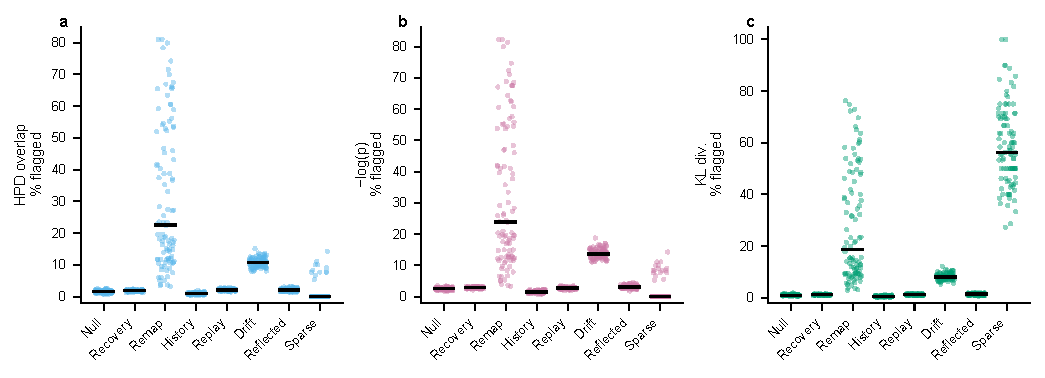
\includegraphics[width=\textwidth]{figures/supplementary/figure03_realizations.pdf}
    \caption{Per-realization flag percentages behind the medians of Fig~\ref{fig:simulation}b. Each panel shows one diagnostic (\textbf{a} HPD overlap, \textbf{b} rank-based predictive $p$-value, \textbf{c} KL divergence); each point is the percentage of spike events flagged in one of the \SimNRealizations{} realizations for the condition on the horizontal axis (horizontal jitter for visibility), and the bar marks the median. The numbers of events per condition and realization are recorded in the summary artifact; the sparse column has a median of \SimSparseEventsMedian{} sparse-cell events per realization.}
    \label{fig:simulation_realizations}
\end{figure}

\begin{figure}[htbp]
    \centering
    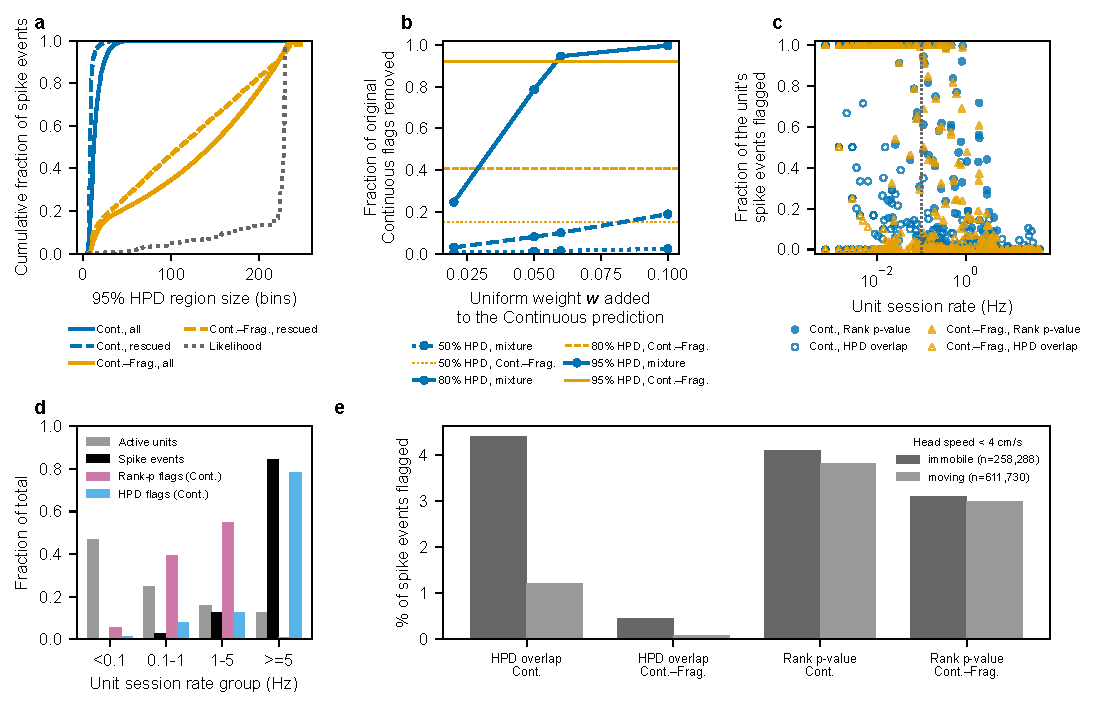
\includegraphics[width=\textwidth]{figures/supplementary/figure04_supplement.pdf}
    \caption{Full-epoch characterization of the Figure~\ref{fig:realdata} flags. \textbf{(a)} Cumulative distributions of the 95\% predictive HPD-region size (in track-interior bins, of \RecNPositionBins) at every spike event (solid) and at the events rescued by the Continuous--Fragmented model (dashed), for the Continuous (blue) and Continuous--Fragmented (orange) models, with the likelihood's 95\% region size (dotted) for comparison. \textbf{(b)} Fraction of the Continuous model's original HPD flags removed when its prediction is replaced by the uniform mixture $(1-w)P_k+wU$ on the same events, as a function of $w$, at 95\% (solid), 80\% (dashed), and 50\% (dotted) coverage; horizontal lines mark the fraction removed by the fitted Continuous--Fragmented model at each coverage. The mixture is a counterfactual applied to the diagnostic's input, not a refitted decoder. \textbf{(c)} Each active unit's session firing rate against the fraction of its spike events flagged by the rank-based $p$-value (filled) and by HPD overlap (open), for both models; the dotted line marks \RecLowRateThresholdHz{} Hz. \textbf{(d)} Fractions of active units, of spike events, and of the Continuous model's rank-based and HPD flags contributed by each firing-rate group. \textbf{(e)} Percentage of events flagged during immobility versus movement (head speed below or above \RecSpeedCutoff{} cm/s) by metric and model. No independent replay labels are available for this epoch.}
    \label{fig:realdata_supplement}
\end{figure}
\clearpage

\section*{Data availability}
The hippocampal recording analyzed here was originally reported by Comrie et al.~\cite{ComrieHippocampalrepresentationsalternative2024} and is available on the Distributed Archives for Neurophysiology Data Integration (DANDI) Archive as dandiset 001942 (\url{https://dandiarchive.org/dandiset/001942}).

\section*{Code availability}
All simulation, analysis, and figure-generation code is publicly available at \url{https://github.com/edeno/statespacecheck-paper}. \textcolor{red}{[TODO: Add the archival DOI (e.g., Zenodo) for the tagged release used in this paper.]}

\section*{Ethical statement}
All animal procedures were approved by the Institutional Animal Care and Use Committee at the University of California, San Francisco (protocol AN174991).

\section*{Acknowledgements}
This work was supported by the National Institutes of Health (RF1MH130623 to U.T.E. and L.M.F. and R01MH136875 to L.M.F.), the Simons Collaboration on the Global Brain (542971 to U.T.E and 521921 and 542981 to L.M.F.), and the Howard Hughes Medical Institute (L.M.F.). A.E.C.\ was supported by the National Science Foundation Graduate Research Fellowship Program (1650113), the National Institutes of Health (F31MH124366), and the UCSF Jonas Cohler Discovery Fellowship.

The authors declare that they have no competing interests.

\section*{Author contributions}

\noindent\textbf{Conceptualization:} UTE, SZ.\par
\noindent\textbf{Methodology:} UTE, SZ.\par
\noindent\textbf{Software:} SZ, ELD.\par
\noindent\textbf{Formal analysis:} SZ, ELD.\par
\noindent\textbf{Investigation:} SZ, UTE, ELD.\par
\noindent\textbf{Data curation:} AEC.\par
\noindent\textbf{Writing -- original draft:} SZ, UTE, ELD.\par
\noindent\textbf{Writing -- review \& editing:} SZ, AEC, LMF, UTE, ELD.\par
\noindent\textbf{Visualization:} SZ, ELD.\par
\noindent\textbf{Supervision:} UTE.\par
\noindent\textbf{Funding acquisition:} UTE, LMF.\par



\bibliographystyle{iopart-num}
\bibliography{Local-GoF-Paper}

\end{document}
